\documentclass[12pt]{article}
%\usepackage{biometrics2}
%\bibliographystyle{asa}
\usepackage[authoryear,round]{natbib}
%\usepackage{times}
\usepackage{amsmath}
\numberwithin{equation}{section}

%% Please use the following statements for
%% managing the text and math fonts for your papers:
\usepackage{times}
%\usepackage[cmbold]{mathtime}
\usepackage{bm}

%\usepackage[plain,noend]{algorithm2e}

\usepackage{mathrsfs}
\usepackage{epsfig,morefloats}
\usepackage{amsfonts}
% \usepackage{showkeys}
%\usepackage{cymacro}
\usepackage{amsthm}
\usepackage{amssymb}
\usepackage{color}
\usepackage{lscape}
\usepackage{rotating}
\usepackage{caption2}
\usepackage{subfigure}
\usepackage{graphicx}
\usepackage{tabularx}

\pagestyle{plain}

%\setlength{\oddsidemargin}{0in} \setlength{\textwidth}{6.4in}
%\setlength{\topmargin}{0in} \setlength{\textheight}{8.25in}
%\setlength{\parindent}{0.2in}

\addtolength{\oddsidemargin}{-.5in}%
\addtolength{\evensidemargin}{-1in}%
\addtolength{\textwidth}{1in}%
\addtolength{\textheight}{1.7in}%
\addtolength{\topmargin}{-1in}%

\def\be{\begin{equation}}
\def\ee{\end{equation}}
\def\bea{\begin{eqnarray}}
\def\eea{\end{eqnarray}}
\def\bd{\begin{displaymath}}
\def\ed{\end{displaymath}}
\def\bda{\begin{eqnarray*}}
\def\eda{\end{eqnarray*}}
\def\bsm{\begin{small}}
\def\esm{\end{small}}

\def\nh{\noindent\hangindent=0.5truecm\hangafter=1}
\def\lsk{\left(}
\def\rsk{\right)}
\def\lbk{\left \{ }
\def\rbk{\right \} }
\def\lmk{\left [ }
\def\rmk{\right ] }

\def\t0{\theta_0}


\def\nn{\nonumber}


\def\kd{\kappa\delta }
\def\ha1{\hat \beta_1}
\def\nr{\nonumber}
\def\ta{\theta_\alpha}
\def\tQ{\tilde Q}
\def\tb{\theta_\beta}
\def\ssi{\sum_{i=1}^n}
\def\ssj{\sum_{j=1}^n}

\newcommand{\bone}{\mbox{\bf 1}}


\def\bnt{\begin{enumerate}}
\def\ent{\end{enumerate}}
\def\T{{ \mathrm{\scriptscriptstyle T} }}
\def\AZ{{ \mathrm{\scriptscriptstyle AZ} }}

\def\AS{A\"{\i}t-Sahalia}
\def\PF{{\bf{Proof}}}

\def\bsc{\begin{scriptsize}}
\def\esc{\end{scriptsize}}
\def\txs{\textstyle}
\def\half{\txs{1\over 2}}

\newtheorem{theorem}{Theorem}
\newtheorem{tmm}{Theorem}[section]
\newtheorem{lemma}{Lemma}
\newtheorem{cy}{Corollary}
\newtheorem{proposition}{Proposition}
\newtheorem{ft}{Fact}[section]
%\theoremstyle{definition}
\newtheorem{as}{Condition}
\newtheorem{ex}{Example}
\newtheorem{example}{Example}
\newtheorem{remark}{Remark}

\newcommand{\calM}{\mathcal{M}}
\newcommand{\calF}{\mathcal{F}}
\newcommand{\calB}{\mathcal{B}}
\newcommand{\E}{\rm E}
\newcommand{\V}{\rm Var}
%\newcommand{\C}{\rm Cov}
\newcommand{\Cor}{\rm Corr}
\newcommand{\Cov}{\rm Cov}

\newcommand{\wh}{\widehat}
\newcommand{\wt}{\widetilde}
\def\spa{\mathrm{span}}
\def\sep{\mathrm{sep}}
\def\thre{\mathrm{thre}}
\def\askip{\vspace{0.1in}}

\makeatletter
\newcommand{\figcaption}{\def\@captype{figure}\caption}
\newcommand{\tabcaption}{\def\@captype{table}\caption}
\makeatother


%%%%%%%%%%%%%%%%%%%%%%%%%%%%%%%%%%%%%%%%%%%%%%%%%%%%
%%%  Abbreviations in math mode                   %%
%%%%%%%%%%%%%%%%%%%%%%%%%%%%%%%%%%%%%%%%%%%%%%%%%%%%
\newcommand{\AR}{{\rm AR}}
\newcommand{\MA}{{\rm MA}}
\newcommand{\ARMA}{{\rm ARMA}}
\newcommand{\AAR}{{\rm AAR}}
\newcommand{\ARIMA}{{\rm ARIMA}}
\newcommand{\FAR}{{\rm FAR}}
\newcommand{\ARCH}{{\rm ARCH}}
\newcommand{\GARCH}{{\rm GARCH}}
\newcommand{\Beta}{{\rm Beta}}
\newcommand{\DLS}{{\mbox{\scriptsize DLS}}}
\newcommand{\IRSC}{{\rm IRSC}}
\newcommand{\IID}{{\rm IID}}
\newcommand{\Leb}{{\rm Leb}}
\newcommand{\LK}{{\mbox{\scriptsize LK}}}
\newcommand{\LKopt}{{\mbox{\scriptsize LK, OPT}}}
\newcommand{\LS}{{\mbox{\scriptsize LS}}}
\newcommand{\LSopt}{{\mbox{\scriptsize LS, OPT}}}
\newcommand{\MISE}{{\rm MISE}}
\newcommand{\MSE}{{\rm MSE}}
\newcommand{\STD}{{\rm STD}}
\newcommand{\MSPE}{{\rm MSPE}}
\newcommand{\MAE}{{\rm MAE}}
\newcommand{\MAD}{{\rm MAD}}
\newcommand{\RSS}{{\rm RSS}}
\newcommand{\WN}{{\rm WN}}
\newcommand{\abias}{{\rm AB}}
%\newcommand{\argmin}{{\rm argmin}}
\newcommand{\avar}{{\rm AV}}
\newcommand{\vech}{{\rm vech}}
\newcommand{\bias}{{\rm Bias}}
\newcommand{\cor}{{\rm Corr}}
\newcommand{\cov}{{\rm Cov}}
\newcommand{\diag}{{\rm diag}}
\newcommand{\etal}{\mbox{\sl et al.\;}}
\newcommand{\ie}{\mbox{\sl i.e.\;}}
\newcommand{\eg}{\mbox{\sl e.g.\;}}
\newcommand{\sgn}{\mbox{sgn}}
\newcommand{\sopt}{\mbox{{\scriptsize opt}}}
\newcommand{\tr}{\mbox{tr}}
\newcommand{\var}{\mbox{Var}}
\newcommand{\C}{\mbox{Cov}}
\newcommand{\AIC}{\mbox{AIC}}
\newcommand{\BIC}{\mbox{BIC}}
\newcommand{\BICP}{\mbox{BICP}}
\newcommand{\BICC}{\mbox{BICC}}
\def\ga{\gamma}
\def\de{\delta}
\def\om{\omega}
\def\la{\lambda}
\def\vphi{\varphi}
\newcommand{\ve}{{\varepsilon}}

%%%%%%%%%%%%%%%%%%%%%%%%%%%%%%%%%%%%%%%%%%%%%%%%%%%%%%
%%%  boldface in math model                         %%
%%%%%%%%%%%%%%%%%%%%%%%%%%%%%%%%%%%%%%%%%%%%%%%%%%%%%%

\newcommand{\bA}{{\mathbf A}}
\newcommand{\bB}{{\mathbf B}}
\newcommand{\bF}{{\mathbf F}}
\newcommand{\bE}{{\mathbf E}}
\newcommand{\bG}{{\mathbf G}}
\newcommand{\bH}{{\mathbf H}}
\newcommand{\bI}{{\mathbf I}}
\newcommand{\bK}{{\mathbf K}}
\newcommand{\bL}{{\mathbf L}}
\newcommand{\bN}{{\mathbf N}}
\newcommand{\bM}{{\mathbf M}}
\newcommand{\bQ}{{\mathbf Q}}
\newcommand{\bP}{{\mathbf P}}
\newcommand{\bR}{{\mathbf R}}
\newcommand{\bS}{{\mathbf S}}
\newcommand{\bT}{{\mathbf T}}
\newcommand{\bU}{{\mathbf U}}
\newcommand{\bV}{{\mathbf V}}
\newcommand{\bW}{{\mathbf W}}
\newcommand{\bX}{{\mathbf X}}
\newcommand{\bY}{{\mathbf Y}}
\newcommand{\bZ}{{\mathbf Z}}
\newcommand{\ba}{{\mathbf a}}
\newcommand{\bb}{{\mathbf b}}
\newcommand{\bfd}{{\mathbf d}}
\newcommand{\bc}{{\mathbf c}}
\newcommand{\bfe}{{\mathbf e}}
\newcommand{\bff}{{\mathbf f}}
\newcommand{\bg}{{\mathbf g}}
\newcommand{\bi}{{\mathbf i}}
\newcommand{\bj}{{\mathbf j}}
%\newcommand{\bm}{{\mathbf m}}
\newcommand{\br}{{\mathbf r}}
\newcommand{\bt}{{\mathbf t}}
\newcommand{\bs}{{\mathbf s}}
\newcommand{\bu}{{\mathbf u}}
\newcommand{\bv}{{\mathbf v}}
\newcommand{\bw}{{\mathbf w}}
\newcommand{\bx}{{\mathbf x}}
\newcommand{\by}{{\mathbf y}}
\newcommand{\bz}{{\mathbf z}}
\newcommand{\balpha} {\boldsymbol{\alpha}}
\newcommand{\bbeta}  {\boldsymbol{\beta}}
\newcommand{\bfeta}  {\boldsymbol{\eta}}
\newcommand{\bvarphi}  {\boldsymbol{\varphi}}
\newcommand{\varphiuv}  {\varphi^{(u,v)}}
\newcommand{\bvphi}  {\boldsymbol{\varphi}}
\newcommand{\bBeta}  {\boldsymbol{\Beta}}
\newcommand{\bdelta} {\boldsymbol{\delta}}
\newcommand{\blambda}{\boldsymbol{\lambda}}
\newcommand{\bepsilonb}{\boldsymbol{\varepsilon}}
\newcommand{\bepsilonbb}{\boldsymbol{\epsilon}}
\newcommand{\bOmega}{\boldsymbol{\Omega}}
\newcommand{\bomega}{\boldsymbol{\omega}}
\newcommand{\bom}{{\boldsymbol{\omega}}}
\newcommand{\bSigma}{\boldsymbol{\Sigma}}
\newcommand{\bsigma}{\boldsymbol{\sigma}}
\newcommand{\bDelta}{\boldsymbol{\Delta}}
\newcommand{\bgamma}{\boldsymbol{\gamma}}
\newcommand{\bga}{\boldsymbol{\gamma}}
\newcommand{\bpi}{\boldsymbol{\pi}}
\newcommand{\bPi}{\boldsymbol{\Pi}}
\newcommand{\bve}{\mbox{\boldmath$\varepsilon$}}
\newcommand{\brho}{\mbox{\boldmath$\rho$}}
\newcommand{\bvarsigma}{\mbox{\boldmath$\varsigma$}}
\newcommand{\bUpsilon}{\boldsymbol{\Upsilon}}
\newcommand{\bTheta} {\boldsymbol{\Theta}}
\newcommand{\bPhi} {\boldsymbol{\Phi}}
\newcommand{\bPsi} {\boldsymbol{\Psi}}
\newcommand{\bRho} {\boldsymbol{\Rho}}
\newcommand{\btheta} {\boldsymbol{\theta}}
\newcommand{\bxi} {\boldsymbol{\xi}}
\newcommand{\bmu} {\boldsymbol{\mu}}
\newcommand{\bzeta} {\boldsymbol{\zeta}}
\newcommand{\bGamma} {\boldsymbol{\Gamma}}
\newcommand{\bLambda} {\boldsymbol{\Lambda}}
\newcommand{\bkappa}{\boldsymbol{\kappa}}
\newcommand{\bC}{{\mathbf C}}
\newcommand{\bD}{{\mathbf D}}
\newcommand{\bzero}{{\mathbf 0}}
\newcommand{\bnu}{\boldsymbol{\nu}}
\newcommand{\diff}{\nabla}
\newcommand{\bXi}{\boldsymbol{\Xi}}
\newcommand{\bchi}{\boldsymbol{\chi}}
\newcommand{\btau}{\boldsymbol{\tau}}

%%%%%%%%%%%%%%%%%%%%%%%%%%%%%%%%%%%%%%%%
%%%  Some useful journal names
%%%%%%%%%%%%%%%%%%%%%%%%%%%%%%%%%%%%%%%%
\def\JRSSB{{\sl Journal of the Royal Statistical Society}, {\bf B}}
\def\JBES{{\sl Journal of Business \& Economic Statistics}}
\def\TRES{{\sl The Review of Economics and Statistics}}
\def\RES{{\sl Review of Economic Studies}}
\def\JRSSA{{\sl Journal of the Royal Statistical Society}, {\bf A}}
\def\JRSSC{{\sl Journal of the Royal Statistical Society}, {\bf C}}
\def\BKA{{\sl Biometrika}}
\def\JASA{{\sl Journal of the American Statistical Association}}
\def\BCS{{\sl Biometrics}}
\def\SS{{\sl Statistica Sinica}}
\def\JAP{{\sl Journal of Applied Probability}}
\def\AAP{{\sl Advances in Applied Probability}}
\def\AS{{\sl The Annals of Statistics}}
\def\JMA{{\sl Journal of multivariate analysis}}
\def\AP{{\sl The Annals of Probability}}
\def\AAP{{\sl The Annals of Applied Probability}}
\def\SPA{{\sl Stochastic Processes and Their Applications}}
\def\TPA{{\sl Theory of Probability and its Applications}}
\def\JSPI{{\sl Journal of Statistical Planning and Inference}}
\def\JNS{{\sl Journal of Nonparametric Statistics}}
\def\ET{{\sl Econometric Theory}}
\def\JOE{{\sl Journal of Econometrics}}
\def\JTSA{{\sl Journal of Time Series Analysis}}
\def\SJS{{\sl Scandinavian Journal of Statistics}}
\def\ISR{{\sl International Statistical Review}}
\def\ANZJS{{\sl Australian \& New Zealand Journal of Statistics}}
\def\JE{{\sl Journal of Econometrics}}
\def\SPL{{\sl Statistics and Probability Letters}}
\def\ZW{{\sl Zeitschrift f{\" u}r Wahrscheinlichkeitstheorie und verwandte Gebiete}}
\def\AMS{{\sl The Annals of Mathematical Statistics}}
\def\PTRF{{\sl Probability Theory and Related Fields}}
\def\JTP{{\sl Journal of Theoretical Probability}}
\def\ECA{{\sl Econometrica}}


%\renewcommand{\baselinestretch}{1.3}
%\hoffset=-0.6in

\begin{document}

\def\spacingset#1{\renewcommand{\baselinestretch}%
{#1}\small\normalsize} \spacingset{1.9}

\title{\Large \bf Supplementary Material to ``Unveiling the Unobservable: Causal Inference on Multiple Derived Outcomes''}

\author{\normalsize Yumou Qiu$^{1}$, Jiarui Sun$^{2}$ and Xiao-Hua Zhou$^{2}$ \\
\normalsize \textit{Iowa State University$^{1}$ and Peking University$^{2}$}}
\date{}
\maketitle


\setcounter{equation}{0}
\def\theequation{S.\arabic{equation}}

\setcounter{section}{0}
\def\thesection{S\arabic{section}}

\setcounter{table}{0}
\renewcommand{\thetable}{S\arabic{table}}

\setcounter{figure}{0}
\renewcommand{\thefigure}{S\arabic{figure}}


In this supplementary file, we first introduce the de-sparsified lasso estimation as a de-biased estimator for regularized regression in Section S1, and show it satisfies the asymptotic unbiasedness condition (Condition 4) for estimating the ATEs on regression coefficients in Example 2.
In Section S2, we verify Condition 4 for sample correlations in Example 1.
The proofs for all theoretical results are provided in Section S3.
Additional simulation and case study results are shown in Figures \ref{simulation3} and \ref{Causalconnection}.

Recall that $\mathcal{X}_i^m(d) = \{\bX_{i, t}(d)\}_{t=1}^{m}$ is the collection of the potential responses $\bX_{i, t}(d)$ for the $i$th subject, 
%and $\epsilon_{i, t, j}(d)$ is the error from the $j$th nodewise regression in Example 2, 
where $\bX_{i, t}(d) = (X_{i, t, 1}(d), \ldots, X_{i, t, p}(d))^{\T}$.
We use $F_{d, i}(\cdot) = F_{d, i}(\cdot, \bT_{i}(d) | \bW_{i})$ to denote the subject level distribution function given all subject level parameters and covariates.
We assume stationary responses so that the mean and covariance of $\bX_{i, t}(d)$ are the same over $t$, where ${\E}_{i}\{\bX_{i, t}(d)\} = \bmu_{i}(d) = (\mu_{i, 1}(d), \ldots, \mu_{i, p}(d))^{\T}$ and ${\V}_{i}\{\bX_{i, t}(d)\} = \bSigma_{i}(d) = (\sigma_{i, j_1j_2}(d))$ for all $t = 1, \ldots, m$, $i = 1, \ldots, n$ and $d = 0, 1$.
%Recall that $\bOmega_{i}(d) = \bSigma_{i}^{-1}(d)$ is the precision matrix of $\bX_{i, t}(d)$.
Here, ${\E}_i(\cdot) = {\E}\{\cdot | \bT_i(d), \bW_i\}$ and ${\V}_i(\cdot) = {\E}\{\cdot | \bT_i(d), \bW_i\}$ denote the mean and variance with respect to the subject level distribution $F_{d, i}(\cdot)$ of the $i$th subject. 
%given $\bT_i(d)$ and $\bW_i$.

Let $C$ be a positive constant which may change from case to case. Let $|\ba|_{\infty} = \max_{j} |a_j|$ for a vector $\ba = (a_1, \ldots, a_p)^{\T}$, and $|\bA|_{\infty} = \max_{j_1, j_2} |a_{j_1j_2}|$ for a matrix $\bA = (a_{j_1j_2})$, which denotes 
%the vector maximum norm for vectors and 
the element-wise maximum norm for vectors and matrices. 


\section{De-biased estimator for regularized regression}
%\label{se:de-bias}

For Example 2, Lasso-type regularized regression is used to estimate the nodewise regression in (2.4) if the dimension $p$ is larger than the subject sample size $m$.
Despite the lasso estimate being consistent under suitable sparsity conditions, it is biased and can not be used to infer the ATEs on regression coefficients. 
In this section, we introduce the de-sparsified lasso estimator \citep{vanderGeerRitov2014, ZZ14}, and verify it satisfies Condition 4.
Let $|\cdot|_1$ and $|\cdot|_2$ denote the $\ell_1$ and $\ell_2$ norm of a vector, respectively.

%In this section, we verify Condition \ref{as:est} under specific cases.  Note that this condition is automatically satisfied if $\hat{Y}_{i,j}(d)$ is an unbiased estimator of $Y_{i,j}(d)$ for $d = 0, 1$ given each subject, for example, the least square estimator of regression coefficients for Example 2 if the $p = o(n)$. We provide sufficient conditions of Condition \ref{as:est} for correlations and regression coefficients in Examples 1 and 2 under high-dimensional and time dependent data.

%Recall that $\mathcal{X}_i^m(d) = \{\bX_{i, t}(d)\}_{t=1}^{m}$ is the collection of the potential responses $\bX_{i, t}(d)$, and $\epsilon_{i, t, j}(d)$ is the error from the $j$th nodewise regression in Example 2, where $\bX_{i, t}(d) = (X_{i, t, 1}(d), \ldots, X_{i, t, p}(d))^{\T}$.
%Suppose the mean and covariance of $\bX_{i, t}(d)$ are the same over $t$ such that ${\E}_{i}\{\bX_{i, t}(d)\} = \bmu_{i}(d) = (\mu_{i, 1}(d), \ldots, \mu_{i, p}(d))^{\T}$ and ${\V}_{i}\{\bX_{i, t}(d)\} = \bSigma_{i}(d) = (\sigma_{i, j_1j_2}(d))$ for all $t = 1, \ldots, m$, $i = 1, \ldots, n$ and $d = 0, 1$. Let $\bOmega_{i}(d) = \bSigma_{i}^{-1}(d)$ be the precision matrix of $\bX_{i, t}(d)$.

Let $\bY_{i, j}^{\ast}(d) = (Y_{i, j 1}^{\ast}(d), \ldots, Y
_{i, j p}^{\ast}(d))^{\T}$ with $Y_{i, j j}^{\ast}(d) = -1$ be the potential coefficients of the $j$th nodewise regression.
Let $\tilde{\bX}_{i, t}(d) = (\tilde{X}_{i, t, 1}(d), \ldots, \tilde{X}_{i, t, p}(d))^{\T}$ and $\tilde{X}_{i, t, j}(d) = X_{i, t, j}(d) - \bar{X}_{i, j}(d)$ be the centered potential responses for the $i$th subject. Let $\tilde{\bY}_{i, j}^{\ast}(d) = (\tilde{Y}_{i, j 1}^{\ast}(d), \ldots, \tilde{Y}
_{i, j p}^{\ast}(d))^{\T}$ be the lasso estimate of the regression coefficients $\bY_{i, j}^{\ast}(d)$, where
$$\tilde{\bY}_{i, j}^{\ast}(d) = \underset{{\bY}_{i, j}^{\ast}(d) \in \mathbb{R}^{p}, {Y}_{i, j j}^{\ast}(d) = -1}{\arg\min} \frac{1}{2m} \sum_{t = 1}^{m}\{ \tilde{\bX}_{i, t}^{\T}(d) {\bY}_{i, j}^{\ast}(d) \}^{2}  + \lambda_{j} |{\bY}_{i, j}^{\ast}(d)|_1 $$
for a penalty parameter $\lambda_{j} > 0$.
%Even though the lasso estimator $\tilde{\bY}_{i, j}^{\ast}(d)$ could be consistent to $\bY_{i, j}^{\ast}(d)$ under suitable conditions, it is a biased estimator. 
To correct the bias of the lasso estimate $\tilde{\bY}_{i, j}^{\ast}(d)$, let
%we consider the de-sparsified lasso estimator. 
%proposed in \cite{vanderGeerRitov2014, ZZ14}.
%Let $\tilde{\bX}_{i, t, -(j_1, j_2)}(d)$ be the sub-vector of $\tilde{\bX}_{i, t}(d)$ without the $j_1$th and $j_2$th elements, and
$$\tilde{\bgamma}_{i, (j_1j_2)}(d) = \underset{\bgamma_{i, (j_1j_2)} \in \mathbb{R}^{p - 2}}{\arg\min} \frac{1}{2m} \sum_{t = 1}^{m} \{\tilde{X}_{i, t, j_2}(d) - \tilde{\bX}_{i, t, -(j_1, j_2)}^{\T}(d) \bgamma_{i, (j_1j_2)}(d) \}^{2} + \lambda_{j_1j_2} | \bgamma_{i, (j_1j_2)}(d)|_{1}$$
be the lasso estimate of regressing $\tilde{X}_{i, t, j_2}(d)$ on $\tilde{\bX}_{i, t, -(j_1, j_2)}(d)$ with a penalty parameter $\lambda_{j_1j_2} > 0$, where $\tilde{\bX}_{i, t, -(j_1, j_2)}(d)$ is the sub-vector of $\tilde{\bX}_{i, t}(d)$ without the $j_1$th and $j_2$th elements.
Following Equation (5) in \cite{vanderGeerRitov2014}, let 
$$\hat{Y}_{i, j_1 j_2}^{\ast}(d) = \tilde{Y}_{i, j_1 j_2}^{\ast}(d) - \frac{1}{m \tilde{a}_{i, j_2j_1}}\sum_{t = 1}^{m}\{\tilde{\bX}_{i, t}^{\T}(d) \tilde{\bY}_{i, j_1}^{\ast}(d)\}\{\tilde{X}_{i, t, j_2}(d) - \tilde{\bX}_{i, t, -(j_1, j_2)}^{\T}(d)\tilde{\bgamma}_{i, (j_1j_2)}(d) \} $$
be the de-sparsified lasso estimator of ${Y}_{i, j_1 j_2}^{\ast}(d)$ for $1 \leq j_1 < j_2 \leq p$, where $$\tilde{a}_{i, j_2j_1} = \frac{1}{m}\sum_{t  = 1}^{m} \tilde{X}_{i, t, j_2}(d) \{\tilde{X}_{i, t, j_2}(d) - \tilde{\bX}_{i, t, -(j_1, j_2)}^{\T}(d)\tilde{\bgamma}_{i, (j_1j_2)}(d) \}.$$
The de-biased estimator for $Y_{i, j_1 j_2}^{\ast}$ can be expressed as $\hat{Y}_{i, j_1 j_2}^{\ast} = D_i \hat{Y}_{i, j_1 j_2}^{\ast}(1) + (1 - D_i) \hat{Y}_{i, j_1 j_2}^{\ast}(0)$.
%In the following, we show $\hat{Y}_{i, j_1 j_2}^{\ast}(d)$ satisfies Condition \ref{as:est} under some conditions. 

Let $\mathscr{F}_{i, 0}^t(d)$ and $\mathscr{F}_{i, t+k}^{\infty}(d)$ be the $\sigma$-fields generated by $\{\bX_{i, u}(d)\}_{u\leq t}$ and $\{\bX_{i, u}(d)\}_{u\geq t+k}$, respectively.
Let
\[
\beta_{i, k}(d) = \sup_t\mathbb{E}_{i}\bigg\{\sup_{B\in\mathscr{F}_{i, t+k}^{\infty}(d)}\big|\mathbb{P}_{i}(B \mid \mathscr{F}_{i, 0}^t(d))-\mathbb{P}_{i}(B)\big|\bigg\}
\]
be the $\beta$-mixing coefficient of the time series $\mathcal{X}_i^m(d)$, where $\mathbb{E}_{i}$ and $\mathbb{P}_{i}$ stand for the expectation and the probability under the subject level distribution $F_{d, i}(\cdot)$ given $\bT_{i}(d)$ and $\bW_i$ of the $i$th subject.
To verify Condition 4 for the de-sparsified lasso estimator $\hat{Y}_{i, j_1 j_2}^{\ast}(d)$ under time-dependent data,
we make the following assumptions.
%sub-Gaussian and $\beta$-mixing conditions on the distribution and dependence of the potential responses $\{\bX_{i, t}(d)\}$ over time. 
%which is formally stated in the following condition.

\medskip

\noindent{\bf Condition S1.}
{\it The responses satisfy 
$\max_{1 \leq i \leq n} \sup_{|\ba|_2 \leq 1} {\E}_{i} \exp [ c_1 \{\ba^{\T} \bX_{i, t}(d)\}^2 ] \leq c_2
%\mbox{ \ and \ } 
%\max_{1 \leq j \leq p} {\E}_{i} \exp \{c_1 \epsilon_{i, t, j}^{2}(d)\} \leq c_2
$ for $d = 0, 1$ and positive constants $c_1$ and $c_2$.
%for $t = 1, \ldots, m$ and $i = 1, \ldots, n$.
}

\medskip

\noindent{\bf Condition S2.}
%The potential responses $\{\mathcal{X}_{i_1}^m(0), \mathcal{X}_{i_1}^m(1)\}$ and $\{\mathcal{X}_{i_2}^m(0), \mathcal{X}_{i_2}^m(1)\}$ are independent from different subjects for $i_1 \neq i_2$ and all $m \geq 1$. 
%Namely, $\{\mathcal{X}_{i_1}(0), \mathcal{X}_{i_1}(1)\}$ and $\{\mathcal{X}_{i_2}(0), \mathcal{X}_{i_2}(1)\}$ are independent for all pairs of subjects with $i_1 \neq i_2$.
{\it The temporal dependence of $\mathcal{X}_{i}^m(d)$ within each subject decays to zero such that $\beta_{i, k}(d) \leq \exp(-c_3 k^{\gamma_0})$ for positive constants $c_3$ and $\gamma_0$ as $k, m \rightarrow\infty$ uniformly for $i = 1, \ldots, n$ and $d = 0, 1$.
}

\medskip

%The responses from different subjects are assumed to be independent with each other, namely, the collections of random variables $\{W_{i_1}, D_{i_1}, X_{i_1, 1}(d) , \ldots, X_{i_1, m}(d)\}$ and $\{W_{i_2}, D_{i_2}, X_{i_2, 1}(d) , \ldots, X_{i_2, m}(d)\}$ observed on the $i_1$th and $i_2$ subjects are independent if $i_1 \neq i_2$.
%But, the observations within the same subject could be dependent among the repeated measurements for $t = 1, \ldots, m$. 
%%We make the following $\beta$-mixing assumption on the dependence of subject response data over time.
%%Let $\mathcal{S}_{\mathcal{V}}$ be the sample space of $\mathcal{V}$.
%Let $\mathscr{F}_{i, 0}^t(d)$ and $\mathscr{F}_{i, t+k}^{\infty}(d)$ be the $\sigma$-fields generated respectively by $\{X_{i, u}(d)\}_{u\leq t}$ and $\{X_{i, u}(d)\}_{u\geq t+k}$.
%Let
%\[ \beta_{i, k}(d) = \sup_t\mathbb{E}_{i}\bigg\{\sup_{B\in\mathscr{F}_{i, t+k}^{\infty}(d)}\big|\mathbb{P}_{i}(B \mid \mathscr{F}_{i, 0}^t(d))-\mathbb{P}_{i}(B)\big|\bigg\} \]
%be the $\beta$-mixing coefficient of the time series $\mathcal{X}_i(d)$, where $\mathbb{E}_{i}$ and $\mathbb{P}_{i}$ stand for the expectation and the probability measure under the distribution of the $i$th subject.
%We make the $\beta$-mixing assumption on the dependence of subject response data $\{\bX_{i, t}(d)\}$ over time, such that $\beta_{i, k}(d)\rightarrow0$ as $k\rightarrow\infty$ uniformly for $i = 1, \ldots, n$ and $d = 0, 1$.

Condition S1 assumes the responses are vector sub-Gaussian distributed, which is a common condition made in studying high-dimensional 
%precision matrices and 
regularized regression \citep{vanderGeerRitov2014, Ning17}. %{qiu2021inference}.
Under Condition S2, the repeated measurements within the same subject are weakly dependent.
The $\beta$-mixing condition is commonly used in time series literature \citep{bradley2005basic}. 
%FanYao_2008}. 
The exponential decay rate is used for the large deviation results of the time series, which is needed to uniformly control the small order terms of the estimators.
A similar condition is made in \cite{ChangQiuYao_2016} for testing high-dimensional precision matrices. 
Notice that the variation of the subject level parameters of interest $\{\bY_{i}(d)\}$ is due to 
%the intrinsic differences among the 
individual heterogeneity in a target population, and the temporal dependence in the responses $\mathcal{X}_i^m(d)$ is caused by the repeated measurement on each subject over time. 
%as a part of the data generation mechanism.
Those are two distinct sources of variation. The strength of the temporal dependence on the repeated measurements can be considered as only related to the time lag $k$ and free of the subject variation.
Therefore, it is reasonable to assume $\beta_{i, k}(d)$ is uniformly bounded for all $i = 1, \ldots, n$ for each given $k$.

%For Example 1 in Section \ref{se:background}, recall that $v_{i, j_1j_2}(d) = \sum_{t = 1}^{m} \{X_{i, t, j_1}(d) - \bar{X}_{i, j_1}(d)\}\{X_{i, t, j_2}(d) - \bar{X}_{i, j_2}(d)\} / m$ is the sample variance of the $i$th subject.
%The sample correlation $\hat{Y}_{i, j_1j_2}(d) = v_{i, j_1j_2}(d) \{v_{i, j_1j_1}(d) v_{i, j_2j_2}(d)\}^{-1/2}$ is the natural estimator of the subject level correlation $Y_{i, j_1j_2}(d)$ for each subject. 
%The following proposition provides a uniform bound on the smaller order term of the sample correlations under time dependent data, and shows that Condition \ref{as:est} is valid for the sample correlations in Example 1.

%\begin{proposition}\label{pn:example1}
%Under Conditions \ref{as:moment} and \ref{as:dependence} and $\log p + \log n = o(m^{c_4})$ for a positive constant $c_4 < 1$, for the sample correlation $\hat{Y}_{i, j_1j_2}(d)$ of each subject, we have ${\E}_{i}\{\hat{Y}_{i, j_1j_2}(d)\} = Y_{i, j_1j_2}(d) + O\{(\log p + \log n) / m\}$ for $i = 1, \ldots, n$ and $d = 0, 1$, where the small order term $O\{(\log p + \log n) / m\}$ is uniform over $1 \leq j_1 < j_2 \leq p$ and $i = 1, \ldots, n$.
%\end{proposition}

%From Proposition \ref{pn:example1}, Condition \ref{as:est} is satisfied for Example 1 as long as $n^{1/2} (\log p + \log n) / m \to 0$ as $n, m, p \to \infty$. This requires the sample size $m$ of each subject being at a higher order than $\sqrt{n}$, but allows an exponential growth of $p$ with respect to $m$.

Let $\tilde{s}_i = \max_{d = 0, 1} \max_{1 \leq j_1 \leq p} \sum_{j_2 \neq j_1} \mathbb{I}\{\omega_{i, j_1j_2}(d) \neq 0\}$ be the $\ell_0$ norm of the precision matrix $\bOmega_{i}(d) = (\omega_{i, j_1j_2}(d))$ of 
$\bX_{i, t}(d)$ for the $i$th subject.
%where $\omega_{i, j_1j_2}(d)$ is the $(j_1, j_2)$th element of $\bOmega_{i}(d)$. 
Let $\tilde{s}_0 = \max_{1 \leq i \leq n} \tilde{s}_i$.
Let $\lambda_{i, \min}(d)$ be the minimum eigenvalue of $\bSigma_{i}(d)$.
The following proposition provides the uniform convergence rate of the expectation of the de-sparsified lasso estimator $\hat{Y}_{i, j_1 j_2}^{\ast}(d)$. 
%and shows that Condition \ref{as:est} 
%is valid for this de-biased estimator of regression coefficients under high-dimensional cases in Example 2.

\medskip

\noindent{\bf Proposition S1.}
{\it Under Conditions S1 and S2, 
if $\log p = o(m^{c_4})$ and $p > n^{c_5}$ for some positive constants $c_4, c_5$,
$\tilde{s}_0 (\log p) = o(m^{1/2})$, the penalty parameters $\lambda_j$ and $\lambda_{j_1j_2}$ being at the order $\{(\log p) / m\}^{1/2}$, and
$\lambda_{i, \min}(d) > c_6^{-1}$ and $\max_{j} \sigma_{i, jj}(d) < c_6$ for a large positive constant $c_6$ and all $i = 1, \ldots, n$,
%for the de-sparisified lasso estimator $\hat{Y}_{i, j_1 j_2}^{\ast}(d)$, 
we have
${\E}_{i}\{\hat{Y}_{i, j_1 j_2}^{\ast}(d)\} = Y^{\ast}_{i, j_1j_2}(d) + O\{ (\tilde{s}_0 \log p) / m\}$ for each subject and $d = 0, 1$, where the small order term $O\{ (\tilde{s}_0 \log p) / m\}$ is uniform over all $i = 1, \ldots, n$ and $1 \leq j_1 < j_2 \leq p$.}

\medskip

Proposition S1 shows the validity of Condition 4 for the de-sparsified lasso estimator in Example 2 if $n^{1/2} \tilde{s}_0 \log p = o(m)$. 
%Similar as the case of treatment effects on correlations,
This relationship between $n$, $m$ and $p$ requires $m$ to be larger than $\sqrt{n}$, and allows an exponential growth rate of $p$.
The conditions on the sparsity and the minimum eigenvalue of $\bSigma_i$ in this proposition are commonly made in the lasso inference literature \citep{vanderGeerRitov2014, Ning17}.


\section{Asymptotic unbiasedness for sample correlation}

We use the sample correlation $\hat{Y}_{i, j_1j_2}(d) = v_{i, j_1j_2}(d) \{v_{i, j_1j_1}(d) v_{i, j_2j_2}(d)\}^{-1/2}$ 
to estimate the subject level correlation of the $i$th subject in Example 1, where $v_{i, j_1j_2}(d) = \sum_{t = 1}^{m} \{X_{i, t, j_1}(d) - \bar{X}_{i, j_1}(d)\}\{X_{i, t, j_2}(d) - \bar{X}_{i, j_2}(d)\} / m$ is the sample covariance.
%The sample correlation $\hat{Y}_{i, j_1j_2}(d) = v_{i, j_1j_2}(d) \{v_{i, j_1j_1}(d) v_{i, j_2j_2}(d)\}^{-1/2}$ is the natural estimator of the subject level correlation $Y_{i, j_1j_2}(d)$ for each subject. 
The following proposition provides a uniform bound on the smaller order term of sample correlations under time-dependent data, and shows that Condition 4 is valid for sample correlations in Example 1.

\medskip

%\begin{proposition}\label{pn:example1}
\noindent{\bf Proposition S2.} {\it
Under Conditions S1 and S2 and $\log p + \log n = o(m^{c_4})$ for a positive constant $c_4 < 1$, for the sample correlation $\hat{Y}_{i, j_1j_2}(d)$ of each subject, we have ${\E}_{i}\{\hat{Y}_{i, j_1j_2}(d)\} = Y_{i, j_1j_2}(d) + O\{(\log p + \log n) / m\}$ for $i = 1, \ldots, n$ and $d = 0, 1$, where the small order term $O\{(\log p + \log n) / m\}$ is uniform over $1 \leq j_1 < j_2 \leq p$ and $i = 1, \ldots, n$.}
%\end{proposition}

\medskip

From Proposition S2, Condition 4 is satisfied for Example 1 as long as $n^{1/2} (\log p + \log n) / m \to 0$ as $n, m, p \to \infty$. This requires the sample size $m$ of each subject to be at a higher order than $\sqrt{n}$, but allows an exponential growth of $p$ with respect to $m$.


\section{Proofs}

\noindent{\bf Proof of Lemma 1.}
Under Condition 3, $D_i$ and $\{\hat{\bY}_{i}(0), \hat{\bY}_{i}(1)\}$ are conditional independent given the covariates, which implies 
${\E}(\hat{\bY}_{i} | D_i = 1, \bW_i) - {\E}(\hat{\bY}_{i} | D_i = 0, \bW_i) = {\E}\{\hat{\bY}_{i}(1) | \bW_i\} - {\E}\{\hat{\bY}_{i}(0) | \bW_i\}$.
%Let $|\cdot|_{\infty}$ denote the element wise maximum norm for a vector, and 
Since ${\E}\{\hat{\bY}_{i}(d) | \bW_i\} = {\E}[{\E}\{\hat{\bY}_{i}(d) | \bT_i(d), \bW_i\} | \bW_i] = {\E}\{\bY_i(d) + \bDelta_{i, m}(d) | \bW_i\}$,
it follows that 
\bea
{\E}\{{\E}(\hat{\bY}_{i} | D_i = 1, \bW_i) - {\E}(\hat{\bY}_{i} | D_i = 0, \bW_i)\} = {\E}\{\bY_{i}(1) - \bY_{i}(0)\} + {\E}\{\bDelta_{i, m}(1) - \bDelta_{i, m}(0)\},
\nn
\eea
where $\bDelta_{i, m}(d) = {\E}\{\hat{\bY}_{i}(d) | \bT_i(d), \bW_i\} - \bY_{i}(d)$.
Therefore, under condition (3.2), we have
$\btau = {\E}\{{\E}(\hat{\bY}_{i} | D_i = 1, \bW_i) - {\E}(\hat{\bY}_{i} | D_i = 0, \bW_i)\}$ as $m \to \infty$. $\square$

\medskip

\noindent{\bf Proof of Proposition 1.}
%Notice that the double subscripts $j_{1}j_{2}$ is used in $Y_{i, j_1j_2}$ and $\tau_{j_1j_2}$ to denote the correlation between $j_1$th and $j_2$th variable in Example 1.
%Here, to unify the notation, we simply use $\hat{Y}_{i, j}$ to denote the $j$th component of $\hat{Y}_{i}$. 
Recall that  $\dot{\rho}_{\beta}(\bW_{i}, D_{i}) = \{D_{i} - \Lambda(\bW_{i}^{\T}\beta)\} \bW_{i}$ is the first derivative of the log likelihood function of the logistic regression, and $\bXi_{\beta_{0}}$ is the inverse of its Fisher information matrix at the true parameter $\bbeta_0$. The MLE $\hat{\bbeta}$ can be expanded as
\begin{equation}
\sqrt{n}\big(\hat{\bbeta} - \bbeta_{0}\big) = \bXi_{\beta_{0}}\frac{1}{\sqrt{n}}\sum_{i=1}^{n}\dot{\rho}_{\beta_{0}}(\bW_{i},D_{i}) + O_{p}(n^{-1/2}).\label{eq:debiasLasso1}
\end{equation}
For each $j$, we can decompose ${\hat{Y}_{i, j}D_{i}} / {\Lambda(\bW_{i}^{\T}\hat{\bbeta})}$ as
\bea
%\frac{\hat{Y}_{i, j_1j_2}D_{i}}{g(\bW_{i}^{\T}\hat{\bbeta})} &=& 
&& \frac{\hat{Y}_{i, j}D_{i}}{\Lambda(\bW_{i}^{\T}\hat{\bbeta})} - \frac{\hat{Y}_{i, j}D_{i}}{\Lambda(\bW_{i}^{\T}\bbeta_{0})} + \frac{\hat{Y}_{i, j}D_{i}}{\Lambda(\bW_{i}^{\T}\bbeta_{0})^{2}}\{\Lambda(\bW_{i}^{\T}\hat{\bbeta}) - \Lambda(\bW_{i}^{\T}\bbeta_{0})\} \label{eq:decomp1} \\
&-& \frac{\hat{Y}_{i, j}D_{i}}{\Lambda(\bW_{i}^{\T}\bbeta_{0})^{2}}\{\Lambda(\bW_{i}^{\T}\hat{\bbeta}) - \Lambda(\bW_{i}^{\T}\bbeta_{0})\} + \frac{\hat{Y}_{i, j}D_{i}}{\Lambda(\bW_{i}^{\T}\bbeta_{0})} \{1 - \Lambda(\bW_{i}^{\T}\bbeta_{0})\} \bW_{i}^{\T}(\hat{\bbeta} - \bbeta_{0}) \ \ \ \ \ \ \label{eq:decomp2} \\
&-& \frac{\hat{Y}_{i, j}D_{i}}{\Lambda(\bW_{i}^{\T}\bbeta_{0})} \{1 - \Lambda(\bW_{i}^{\T}\bbeta_{0})\} (\bW_{i}^{\T}\hat{\bbeta} - \bW_{i}^{\T}\bbeta_{0}) \nn \\
&& \ \ \ \ \ \ \ \ \ \ \ \ \ + \ \frac{1}{n}\sum_{k = 1}^{n}  \frac{\hat{Y}_{i, j}D_{i}}{\Lambda(\bW_{i}^{\T}\bbeta_{0})} \{1 - \Lambda(\bW_{i}^{\T}\bbeta_{0})\} \bW_{i}^{\T} 
\bXi_{\beta_{0}}\dot{\rho}_{\beta_{0}}(\bW_{k},D_{k})
%\mathcal{I}^{-1} \ell^{(1)}(D_{k}, \bW_{k}, \beta_{0}) 
\label{eq:decomp3} \\
&+& \frac{\hat{Y}_{i, j}D_{i}}{\Lambda(\bW_{i}^{\T}\bbeta_{0})} - \frac{1}{n}\sum_{k = 1}^{n}  \frac{\hat{Y}_{i, j}D_{i}}{\Lambda(\bW_{i}^{\T}\bbeta_{0})} \{1 - \Lambda(\bW_{i}^{\T}\bbeta_{0})\} \bW_{i}^{\T} 
\bXi_{\beta_{0}}\dot{\rho}_{\beta_{0}}(\bW_{k},D_{k})
%\mathcal{I}^{-1} \ell^{(1)}(D_{k}, \bW_{k}, \beta_{0}). 
\label{eq:decomp4}
\eea
Since $Y_{i,j}$ and $\bW_{i}^{\T}\bbeta_{0}$ are bounded for all $i$ and $j$, 
by Taylor expansion and the expansion of $\hat{\bbeta}$ from (\ref{eq:debiasLasso1}), it can be shown that (\ref{eq:decomp1}), (\ref{eq:decomp2}) and  (\ref{eq:decomp3}) are uniformly bounded at the order $O_p(n^{-1})$ for all $i = 1, \ldots, n$ and $j = 1, \ldots, p_0$.
%(\ref{eq:MLEExpansion}).
This leads to 
$$\frac{\hat{Y}_{i, j}D_{i}}{\Lambda(\bW_{i}^{\T}\hat{\bbeta})} = \frac{\hat{Y}_{i, j}D_{i}}{\Lambda(\bW_{i}^{\T}\bbeta_{0})} - \frac{1}{n}\sum_{k = 1}^{n} \frac{\hat{Y}_{i, j}D_{i}}{\Lambda(\bW_{i}^{\T}\bbeta_{0})} \{1 - \Lambda(\bW_{i}^{\T}\bbeta_{0})\} \bW_{i}^{\T} 
\bXi_{\beta_{0}}\dot{\rho}_{\beta_{0}}(\bW_{k},D_{k}) + O_{p}(n^{-1})$$
uniformly for all $i$ and $j$.
Similar result also holds for $\hat{Y}_{i, j}(1 - D_{i}) / \{1 - \Lambda(\bW_{i}^{\T}\bbeta_{0})\}$.
Therefore,
\bea
%&&
%\frac{1}{n}\sum_{i = 1}^{n}\bigg\{\frac{\hat{Y}_{i, j}D_{i}}{\Lambda(\bW_{i}^{\T}\hat{\bbeta})} - \frac{\hat{Y}_{i, j}(1 - D_{i})}{1 - \Lambda(\bW_{i}^{\T}\hat{\bbeta})}\bigg\} \nn \\
\hat{\tau}_{j} = 
\frac{1}{n}\sum_{i = 1}^{n}\bigg\{\frac{\hat{Y}_{i, j}D_{i}}{\Lambda(\bW_{i}^{\T}\bbeta_{0})} - \frac{\hat{Y}_{i, j}(1 - D_{i})}{1 - \Lambda(\bW_{i}^{\T}\bbeta_{0})}\bigg\} - \hat{\mathcal{H}}_{j} \frac{1}{n}\sum_{k = 1}^{n} \bXi_{\beta_{0}}\dot{\rho}_{\beta_{0}}(\bW_{k},D_{k}) + O_{p}(n^{-1}), \nn
\eea
where 
$$\tilde{\mathcal{H}}_{j} = 
\frac{1}{n}\sum_{i = 1}^{n}\bigg\{\frac{1 - \Lambda(\bW_{i}^{\T}\bbeta_{0})}{\Lambda(\bW_{i}^{\T}\bbeta_{0})} \hat{Y}_{i, j}D_{i} + \frac{\Lambda(\bW_{i}^{\T} \bbeta_{0})}{1 - \Lambda(\bW_{i}^{\T} \bbeta_{0})} \hat{Y}_{i, j}(1 - D_{i}) \bigg\} \bW_{i}^{\T}.$$

Recall that $\mathcal{H} = {\E}\big( \big[ \{1 - \Lambda(\bW_{i}^{\T}\bbeta_{0})\} \bY_{i}(1) + \Lambda(\bW_{i}^{\T}\bbeta_{0})\bY_{i}(0) \big] \bW_{i}^{\T} \big)$. 
%and $Y(d, w) = {\E}\{\bY_{i}(d) \mid \bW_{i} = w\}$.
Let 
$$\tilde{\mathcal{H}} = 
\frac{1}{n}\sum_{i = 1}^{n}\bigg\{\frac{1 - \Lambda(\bW_{i}^{\T}\bbeta_{0})}{\Lambda(\bW_{i}^{\T}\bbeta_{0})} \hat{\bY}_{i}D_{i} + \frac{\Lambda(\bW_{i}^{\T} \bbeta_{0})}{1 - \Lambda(\bW_{i}^{\T} \bbeta_{0})} \hat{\bY}_{i}(1 - D_{i}) \bigg\} \bW_{i}^{\T}.$$
Then, $\tilde{\mathcal{H}}_{j}$ is the $j$th row of $\tilde{\mathcal{H}}$. 
Note that ${\E}\{\hat{Y}_{i, j}(d)|\bW_i\} = {\E}\{Y_{i, j}(d)|\bW_i\} + {\E}\{\Delta_{i, j, m}(d)|\bW_i\}$ for $d = 0, 1$, and ${\E}\{|\Delta_{i, j, m}(d)|\} = O(\delta_m)$ under Condition 4.
It follows that
\bea
&&{\E}\bigg\{\frac{1 - \Lambda(\bW_{i}^{\T}\bbeta_{0})}{\Lambda(\bW_{i}^{\T}\bbeta_{0})} \hat{Y}_{i, j}D_{i} + \frac{\Lambda(\bW_{i}^{\T} \bbeta_{0})}{1 - \Lambda(\bW_{i}^{\T} \bbeta_{0})} \hat{Y}_{i, j}(1 - D_{i}) \bigg\} \bW_{i} \nn \\
&=& 
{\E}\big( \big[ \{1 - \Lambda(\bW_{i}^{\T}\bbeta_{0})\}{\E}\{\hat{Y}_{i,j}(1) | \bW_i\} + \Lambda(\bW_{i}^{\T} \bbeta_{0}) {\E}\{\hat{Y}_{i,j}(0) | \bW_i\} \big] \bW_{i} \big) \nn \\
&=&
{\E}\big( \big[ \{1 - \Lambda(\bW_{i}^{\T}\bbeta_{0})\}Y_{i,j}(1) + \Lambda(\bW_{i}^{\T} \bbeta_{0}) Y_{i,j}(0) \big] \bW_{i} \big) + B_{1, m}, \nn
\eea
where $B_{1, m} = {\E}\big( \big[ \{1 - \Lambda(\bW_{i}^{\T}\bbeta_{0})\}{\E}\{\Delta_{i,j,m}(1) | \bW_i\} + \Lambda(\bW_{i}^{\T} \bbeta_{0}) {\E}\{\Delta_{i,j,m}(0) | \bW_i\} \big] \bW_{i} \big)$.
We have $|B_{1, m}| \leq C {\E}\big( {\E}\{|\Delta_{i,j,m}(1)| | \bW_i\} + {\E}\{|\Delta_{i,j,m}(0)| | \bW_i\} \big) \leq C({\E}|\Delta_{i,j,m}(1)| + {\E}|\Delta_{i,j,m}(0)|) = O(\delta_m)$.
Since the summation terms in $\tilde{\mathcal{H}}_{j}$ are independent, 
%where ${\E}_i(\cdot)$ denotes the conditional expectation given the covariates $\bW_i$ and the subject level parameters $Y_{i}$.
%where $Y_j(d, w) = {\E}\{Y_{i,j}(d) | \bW_i = w\}$ is the $j$th component of $Y(d, w)$ for $d = 0, 1$, 
by the large deviation results \citep{petrov2012sums}, we have that $|\tilde{\mathcal{H}} - \mathcal{H}|_{\infty} = O_p\{(\log p_0)^{1/2}n^{-1/2} + \delta_m\}$. Therefore, 
\bea
\hat{\tau}_{j} - \tau_{j}
&=& 
\frac{1}{n}\sum_{i = 1}^{n} \tilde{\eta}_{ij}
%\frac{1}{n}\sum_{i = 1}^{n}\bigg\{\frac{\hat{Y}_{i, j}D_{i}}{\Lambda(\bW_{i}^{\T}\bbeta_{0})} - \frac{\hat{Y}_{i, j}(1 - D_{i})}{1 - \Lambda(\bW_{i}^{\T}\bbeta_{0})}\bigg\} - \mathcal{H}_{j} \frac{1}{n}\sum_{k = 1}^{n} \bXi_{\beta_{0}}\dot{\rho}_{\beta_{0}}(\bW_{k},D_{k}) \nn \\
+ 
O_{p}\{(\log p_0)^{1/2}n^{-1} + \delta_m n^{-1/2}\},\label{eq:tauhat}
\eea
where 
\bea
\tilde{\eta}_{ij} &=& \frac{\hat{Y}_{i, j}D_{i}}{\Lambda(\bW_{i}^{\T}\bbeta_{0})} - \frac{\hat{Y}_{i, j}(1 - D_{i})}{1 - \Lambda(\bW_{i}^{\T}\bbeta_{0})} - \mathcal{H}_{j} \bXi_{\beta_{0}} \{D_{i} - \Lambda(\bW_{i}^{\T}\bbeta_{0})\} \bW_{i} - \tau_j, 
%\label{eq:hateta}
\nn\eea
is defined in (4.6), $\mathcal{H}_{j}$ is the $j$th row of $\mathcal{H}$, and the small order term 
%$O_{p}\{(\log p_0)^{1/2}n^{-1} + \delta_m n^{-1/2}\}$ 
in (\ref{eq:tauhat})
is uniform over all $j = 1, \ldots, p_0$. 

Let $\tilde{\bfeta}_i = (\tilde{\eta}_{i1}, \ldots, \tilde{\eta}_{i p_0})^{\T}$ and $\check{\bfeta}_i = (\check{\eta}_{i1}, \ldots, \check{\eta}_{i p_0})^{\T}$ where $\check{\eta}_{ij} = \tilde{\eta}_{ij} - {\E}(\tilde{\eta}_{ij})$. %Since ${\E}\{\hat{Y}_{i,j}(d) | \bW_i\} = {\E}\{Y_{i,j}(d) | \bW_i\} + \delta_m$ for $d = 0, 1$ 
Under Conditions 3 and 4, it follows that
$${\E}(\tilde{\eta}_{ij}) = {\E}\big[ {\E}\big\{\hat{Y}_{i,j}(1) | \bW_i\} - {\E}\big\{\hat{Y}_{i,j}(0) | \bW_i\} \big] - \tau_j = {\E}\{\Delta_{i, j, m}(1) - \Delta_{i, j, m}(0)\} =  O(\delta_m).$$
This leads to
%Under Conditions \ref{as:UCF} and \ref{as:est}. Therefore, 
$$\hat{\tau}_{j} - \tau_{j}
= 
\frac{1}{n}\sum_{i = 1}^{n} \check{\eta}_{ij}
%\frac{1}{n}\sum_{i = 1}^{n}\bigg\{\frac{\hat{Y}_{i, j}D_{i}}{\Lambda(\bW_{i}^{\T}\beta_{0})} - \frac{\hat{Y}_{i, j}(1 - D_{i})}{1 - \Lambda(\bW_{i}^{\T}\beta_{0})}\bigg\} - \mathcal{H}_{j} \frac{1}{n}\sum_{k = 1}^{n} \bXi_{\beta_{0}}\dot{\rho}_{\beta_{0}}(\bW_{k},D_{k}) \nn \\
+ 
O_{p}\{(\log p_0)^{1/2}n^{-1} + \delta_m n^{-1/2} + \delta_m\},$$
where $\{\check{\eta}_{ij}\}_{i = 1}^{n}$ are independent mean zero sequence, and the small order term is uniform over all $j = 1, \ldots, p_0$.
This finishes the proof of Proposition 1. $\square$

\iffalse
%Let $\bar{\xi}_{i} = \bar{\xi}_{i}(1) D_{i} + \bar{\xi}_{i}(0) (1 - D_{i})$.
Note that $\hat{Y}_{i, j} = Y_{i, j} + \bar{\xi}_{i, j} + O_{p}\{\log(p_0) / m\}$ under Condition \ref{as:est}, where $\bar{\xi}_{i, j} =  D_{i} \bar{\xi}_{i, j}(1) + (1 - D_{i}) \bar{\xi}_{i, j}(0)$. Since $\bar{\xi}_{i, j}(d)$ is independent of $D_{i}$ given $\bW_{i}$ under Condition \ref{as:UCF}, we have ${\E}\{\bar{\xi}_{i, j}D_{i} / \Lambda(\bW_{i}^{\T}\bbeta_{0})\} = {\E}\{\bar{\xi}_{i, j}(1)\} = 0$. 
Under Condition \ref{as:est}, from concentration inequalities and $\max_{i, j}{\V}\{\bar{\xi}_{i,j}(d)\} \leq m^{-c_1}$ for a positive constant $c_1$, it can be shown that $$\max_{j} \bigg| \frac{1}{n}\sum_{i = 1}^{n} \frac{\bar{\xi}_{i, j} D_{i}}{\Lambda(\bW_{i}^{\T}\bbeta_{0})} \bigg| = O_{p}\{\log(p_0)n^{-1/2}m^{-c_1/2}\},$$
which implies that
\bea
\frac{1}{n}\sum_{i = 1}^{n} \frac{\hat{Y}_{i, j}D_{i}}{\Lambda(\bW_{i}^{\T}\bbeta_{0})} 
%&=& \frac{1}{n}\sum_{i = 1}^{n} \frac{(Y_{i, j} + \bar{\xi}_{i, j})D_{i}}{\Lambda(\bW_{i}^{\T}\bbeta_{0})} + O_{p}(m^{-1}) \nn \\
&=& \frac{1}{n}\sum_{i = 1}^{n} \frac{Y_{i, j} D_{i}}{\Lambda(\bW_{i}^{\T}\bbeta_{0})} + O_{p}\{\log(p_0) / m\} + O_{p}\{\log(p_0)n^{-1/2}m^{-c_1/2}\}. \nn
\eea
Similarly, up to a smaller order term $O_{p}\{\log(p_0) / m\} + O_{p}\{\log(p_0)n^{-1/2}m^{-c_1/2}\}$, it can be shown that 
\bea
&&\frac{1}{n}\sum_{i = 1}^{n}\frac{\hat{Y}_{i, j}(1 - D_{i})}{1 - \Lambda(\bW_{i}^{\T}\bbeta_{0})} = \frac{1}{n}\sum_{i = 1}^{n}\frac{Y_{i, j}(1 - D_{i})}{1 - \Lambda(\bW_{i}^{\T}\bbeta_{0})} \mbox{ \ and } \nn \\
&&\hat{\mathcal{H}}_{j} = \frac{1}{n}\sum_{i = 1}^{n}\bigg\{\frac{1 - \Lambda(\bW_{i}^{\T}\bbeta_{0})}{\Lambda(\bW_{i}^{\T}\bbeta_{0})} Y_{i, j}D_{i} + \frac{\Lambda(\bW_{i}^{\T} \bbeta_{0})}{1 - \Lambda(\bW_{i}^{\T} \bbeta_{0})} Y_{i, j}(1 - D_{i}) \bigg\} \bW_{i}^{\T}. \nn
\eea
It follows that $\hat{\mathcal{H}}_{j} = \mathcal{H}_{j} + O_{p}\{\log(p_0) n^{-1/2}\} + O_{p}\{\log(p_0) / m\}$,
%\be
%\hat{\mathcal{H}}_{j} = \frac{1}{n}\sum_{i = 1}^{n}\bigg\{\frac{1 - \Lambda(\bW_{i}^{\T}\beta_{0})}{\Lambda(\bW_{i}^{\T}\beta_{0})} Y_{i, j}D_{i} + \frac{\Lambda(\bW_{i}^{\T} \beta_{0})}{1 - \Lambda(\bW_{i}^{\T} \beta_{0})} Y_{i, j}(1 - D_{i}) \bigg\} \bW_{i}^{\T} = \mathcal{H}_{j} + O_{p}(n^{-1/2}), \nn
%\ee
where $\mathcal{H}_{j}$ is the $j$th row of $\mathcal{H}$.
Those results lead to
\bea
\hat{\tau}_{j} &=& 
\frac{1}{n}\sum_{i = 1}^{n}\bigg\{\frac{Y_{i, j}D_{i}}{\Lambda(\bW_{i}^{\T}\bbeta_{0})} - \frac{Y_{i, j}(1 - D_{i})}{1 - \Lambda(\bW_{i}^{\T}\bbeta_{0})}\bigg\} - \mathcal{H}_{j}^{\T} \frac{1}{n}\sum_{i = 1}^{n} \bXi_{\beta_{0}}\dot{\rho}_{\beta_{0}}(\bW_{i},D_{i}) \nn \\
&+& O_{p}\{\log(p_0)(n^{-1} + m^{-1})\} + O_{p}\{\log(p_0)n^{-1/2}m^{-c_1/2}\}, \nn
\eea
where the small order terms are uniform for all $j = 1, \ldots, p_0$.
This finishes the proof of Proposition \ref{pn:1}. $\square$
\fi

\iffalse
Let $M_{i, t, j_1j_2}(d) = \{X_{i, t, j_1}(d) - \mu_{i, j_1}(d)\}\{X_{i, t, j_2}(d) - \mu_{i, j_2}(d)\} - \sigma_{i, j_1j_2}(d)$.
For the subject level correlation estimates, we have
\be\begin{split}
&\hat{Y}_{i, j_1j_2}(d) - Y_{i, j_1j_2}(d) = \frac{1}{m}\sum_{t = 1}^{m}\eta_{i, t, j_1j_2}(d) + O_{p}(m^{-1}) \mbox{ \ for} \\
\eta_{i, t, j_1j_2}(d)& = \frac{M_{i, t, j_1j_2}(d)}{\{\sigma_{i, j_1j_1}(d)\sigma_{i, j_2j_2}(d)\}^{1/2}} - \frac{Y_{i, j_1j_2}(d) }{2\sigma_{i, j_1j_1}(d)}M_{i, t, j_1j_1}(d) - \frac{Y_{i, j_1j_2}(d) }{2\sigma_{i, j_2j_2}(d)}M_{i, t, j_2j_2}(d).
\end{split}\label{eq:rhoExpansion} \ee
We have $\frac{1}{n}\sum_{i = 1}^{n}\frac{1 - g(\bW_{i}^{\T}\bbeta_{0})}{g(\bW_{i}^{\T}\bbeta_{0})} \hat{Y}_{i, j_1j_2}D_{i} \bW_{i}^{\T} = \mathcal{H}_{1, j_1j_2} + O_{p}(n^{-1/2}) + O_{p}(m^{-1/2})$.
By the independence of $\eta_{i, t, j_1j_2}$ and $D_{i}$ given $\bW_{i}$, it follows that

\be
%\begin{split}
\mathcal{H}_{1, j_1j_2} = {\E} \bigg\{ \frac{1 - \Lambda(\bW_{i}^{\T}\bbeta_{0})}{\Lambda(\bW_{i}^{\T}\bbeta_{0})} Y_{i, j_1j_2}D_{i} \bW_{i}^{\T} \bigg\} \mbox{ \ and \ } 
\mathcal{H}_{2, j_1j_2} = {\E} \bigg\{ \frac{\Lambda(\bW_{i}^{\T}\bbeta_{0})}{1 - \Lambda(\bW_{i}^{\T}\bbeta_{0})} Y_{i, j_1j_2}(1 - D_{i}) \bW_{i}^{\T} \bigg\}.
%\end{split}
%\label{eq:HMatrix}
\nn\ee
\fi

\medskip
\noindent{\bf Proof of Proposition 2.} To calculate the variance of $\hat{\tau}_j$, by the expansion (\ref{eq:tauhat}) and the independence of $\{\tilde{\eta}_{ij}\}$ among subjects, it suffices to consider the variance of $\tilde{\eta}_{ij}$.
Recall that  
$$\theta_j = \frac{1}{n} \sum_{i = 1}^{n} {\E}\bigg[ \bigg\{\frac{\hat{Y}_{i, j}D_{i}}{\Lambda(\bW_{i}^{\T}\bbeta_{0})} - \frac{\hat{Y}_{i, j}(1 - D_{i})}{1 - \Lambda(\bW_{i}^{\T}\bbeta_{0})}  - \tau_j \bigg\} - \mathcal{H}_{j} \bXi_{\beta_{0}} \{D_{i} - \Lambda(\bW_{i}^{\T}\bbeta_{0})\} \bW_{i} \bigg]^{2}$$
is defined in (4.7).
From the proof of Proposition 1, we have ${\V}\{n^{1/2}(\hat{\tau}_j - \tau_j)\} = \theta_j + o(1)$
if $(\log p_0) / n = o(1)$ and $n^{1/2} \delta_{m} = o(1)$.

We first derive the expression of $\theta_j$ in terms of $Y_{i, j}(d)$.
Similar as bounding the small order term $B_{1, m}$ in the proof of Proposition 1, we have
$$
{\E}\bigg[ \frac{\hat{Y}_{i, j}D_{i}}{\Lambda(\bW_{i}^{\T}\bbeta_{0})} \mathcal{H}_{j} \bXi_{\beta_{0}} \{D_{i} - \Lambda(\bW_{i}^{\T}\bbeta_{0})\} \bW_{i} \bigg]
%&=&
%{\E}\bigg[ \frac{\hat{Y}_{i, j}(1)D_{i}}{\Lambda(\bW_{i}^{\T}\bbeta_{0})} \mathcal{H}_{j} \bXi_{\beta_{0}} \{1 - \Lambda(\bW_{i}^{\T}\bbeta_{0})\} \bW_{i} \bigg] \nn \\
%&=&
=
{\E}\big[ Y_{i, j}(1) \mathcal{H}_{j} \bXi_{\beta_{0}} \{1 - \Lambda(\bW_{i}^{\T}\bbeta_{0})\} \bW_{i} \big] + O(\delta_m), 
$$
and 
$$
{\E}\bigg[ \frac{\hat{Y}_{i, j}(1 - D_{i})}{1 - \Lambda(\bW_{i}^{\T}\bbeta_{0})} \mathcal{H}_{j} \bXi_{\beta_{0}} \{D_{i} - \Lambda(\bW_{i}^{\T}\bbeta_{0})\} \bW_{i} \bigg] 
=
- {\E}\big[ Y_{i, j}(0) \mathcal{H}_{j} \bXi_{\beta_{0}} \Lambda(\bW_{i}^{\T}\bbeta_{0}) \bW_{i} \big] + O(\delta_m).
$$
%To simplify notations, let ${\E}_i(\cdot) = {\E}\{\cdot | \bT_i(d), \bW_i\}$ and ${\V}_i(\cdot) = {\E}\{\cdot | \bT_i(d), \bW_i\}$ denote the expectation and variance with respect to the distribution $F_{d, i}(\cdot)$ given all the subject level random effects of the $i$th subject.
Since ${\E}_i\{\hat{Y}_{i, j}^2(d)\} = {\V}_i\{\hat{Y}_{i, j}(d)\} + {\E}_i^2\{\hat{Y}_{i, j}(d)\} = {\V}_i\{\hat{Y}_{i, j}(d)\} + Y_{i,j}^2(d) + \Delta_{i, j, m}^2(d) + 2 \Delta_{i, j, m}(d) Y_{i,j}(d)$, 
it follows that ${\E}\{\hat{Y}_{i, j}^2(d) | \bW_i\} = {\E}[{\V}_i\{\hat{Y}_{i, j}(d)\} | \bW_i] + {\E}\{Y_{i, j}^2(d) | \bW_i\} + {\E}\{\Delta_{i, j, m}^2(d) | \bW_i\} + 2 {\E}\{\Delta_{i, j, m}(d) Y_{i,j}(d) | \bW_i\}$.
This implies that 
\bea
&&{\E}\bigg\{\frac{\hat{Y}_{i, j}D_{i}}{\Lambda(\bW_{i}^{\T}\bbeta_{0})} - \frac{\hat{Y}_{i, j}(1 - D_{i})}{1 - \Lambda(\bW_{i}^{\T}\bbeta_{0})}  - \tau_j \bigg\}^2 \nn \\
&=&
{\E}\bigg\{\frac{\hat{Y}_{i, j}D_{i}}{\Lambda(\bW_{i}^{\T}\bbeta_{0})} - \frac{\hat{Y}_{i, j}(1 - D_{i})}{1 - \Lambda(\bW_{i}^{\T}\bbeta_{0})} \bigg\}^2 - \tau_j^2  + O(\delta_m) \nn \\
&=&
{\E}\bigg[\frac{\hat{Y}_{i, j}^2D_{i}}{\Lambda^2(\bW_{i}^{\T}\bbeta_{0})} + \frac{\hat{Y}_{i, j}^2(1 - D_{i})}{\{1 - \Lambda(\bW_{i}^{\T}\bbeta_{0})\}^2} \bigg] - \tau_j^2  + O(\delta_m), \nn 
\eea
where
\bea
{\E}\bigg[ \frac{\hat{Y}_{i, j}^2D_{i}}{\Lambda^2(\bW_{i}^{\T}\bbeta_{0})} \bigg]
&=& 
{\E}\bigg[\frac{Y_{i, j}^2(1) + {\V}_i\{\hat{Y}_{i, j}(1)\} + \Delta_{i, j, m}^2(d) + 2\Delta_{i, j, m}(d) Y_{i,j}(d)}{\Lambda(\bW_{i}^{\T}\bbeta_{0})} \bigg] \nn \\ 
&=& 
{\E}\bigg[\frac{Y_{i, j}^2(1) + {\V}_i\{\hat{Y}_{i, j}(1)\}}{\Lambda(\bW_{i}^{\T}\bbeta_{0})} \bigg] + O(\delta_m),\nn
\eea
as $|{\E}\{\Delta_{i, j, m}(d) Y_{i,j}(d) / \Lambda(\bW_{i}^{\T}\bbeta_{0})\}| \leq C {\E}|\Delta_{i, j, m}(d)| = O(\delta_m)$ and ${\E}\{\Delta_{i, j, m}^2(d) / \Lambda(\bW_{i}^{\T}\bbeta_{0})\} \leq C {\E}|\Delta_{i, j, m}(d)| = O(\delta_m)$.
Similarly, we can show 
\bea
{\E}\bigg[\frac{\hat{Y}_{i, j}^2(1 - D_{i})}{\{1 - \Lambda(\bW_{i}^{\T}\bbeta_{0})\}^2} \bigg]
&=&
{\E}\bigg[\frac{Y_{i, j}^2(0) + {\V}_i\{\hat{Y}_{i, j}(0)\}}{1 - \Lambda(\bW_{i}^{\T}\bbeta_{0})}\bigg] + O(\delta_m).
\nn
\eea
Therefore, we have
\bea
&&{\E}\bigg\{\frac{\hat{Y}_{i, j}D_{i}}{\Lambda(\bW_{i}^{\T}\bbeta_{0})} - \frac{\hat{Y}_{i, j}(1 - D_{i})}{1 - \Lambda(\bW_{i}^{\T}\bbeta_{0})}  - \tau_j \bigg\}^2 \nn \\
&=& 
{\E}\bigg[\frac{Y_{i, j}^2(1) + {\V}_i\{\hat{Y}_{i, j}(1)\}}{\Lambda(\bW_{i}^{\T}\bbeta_{0})} + 
\frac{Y_{i, j}^2(0) + {\V}_i\{\hat{Y}_{i, j}(0)\}}{1 - \Lambda(\bW_{i}^{\T}\bbeta_{0})}\bigg] - \tau_j^2 + O(\delta_m), \nn 
\eea
which includes both the subject heterogeneity variation and the estimation variation ${\V}_i\{\hat{Y}_{i, j}(d)\}$ of $\hat{Y}_{i, j}(d)$ given the subject level parameters. 
Combining the above terms together, we have
\bea
\theta_j &=& 
\frac{1}{n} \sum_{i = 1}^{n}
{\E}\bigg[\frac{Y_{i, j}^2(1) + {\V}_i\{\hat{Y}_{i, j}(1)\}}{\Lambda(\bW_{i}^{\T}\bbeta_{0})} + 
\frac{Y_{i, j}^2(0) + {\V}_i\{\hat{Y}_{i, j}(0)\}}{1 - \Lambda(\bW_{i}^{\T}\bbeta_{0})}\bigg] \nn \\
&-& 
2{\E}\big( [Y_{i, j}(1) \{1 - \Lambda(\bW_{i}^{\T}\bbeta_{0})\} + Y_{i, j}(0)\Lambda(\bW_{i}^{\T}\bbeta_{0})] \mathcal{H}_{j} \bXi_{\beta_{0}} \bW_{i} \big) \nn \\
&+&
{\E}[\mathcal{H}_{j} \bXi_{\beta_{0}} \{D_{i} - \Lambda(\bW_{i}^{\T}\bbeta_{0})\} \bW_{i}]^2
- \tau_j^2 + O(\delta_m). \label{eq:theta-expansion}
\eea

Next, we show the consistency of the estimator $\hat{\theta}_{j} = \sum_{i = 1}^{n} \hat{\eta}_{ij}^2 / n$ of $\theta_j$, where
\be
\hat{\eta}_{ij} = 
\frac{\hat{Y}_{i, j}D_{i}}{\Lambda(\bW_{i}^{\T}\hat{\bbeta})} 
- \frac{\hat{Y}_{i, j}(1 - D_{i})}{1 - \Lambda(\bW_{i}^{\T}\hat{\bbeta})} - \hat{\tau}_{j} - \hat{\mathcal{H}}_{j} \hat{\mathcal{I}}^{-1} \{D_{i} - \Lambda(\bW_{i}^{\T}\hat{\bbeta})\} \bW_{i}
\nn\ee
as defined in (4.8), $\hat{\mathcal{H}}_{j}$ is the $j$th row of $\hat{\mathcal{H}}$ and 
$$
\hat{\mathcal{H}} = \frac{1}{n}\sum_{i = 1}^{n} \bigg\{ \frac{1 - \Lambda(\bW_{i}^{\T}\hat{\bbeta})}{\Lambda(\bW_{i}^{\T}\hat{\bbeta})} D_{i} + \frac{\Lambda(\bW_{i}^{\T}\hat{\bbeta})}{1 - \Lambda(\bW_{i}^{\T}\hat{\bbeta})} (1 - D_{i})\bigg\} \hat{\bY}_{i}\bW_{i}^{\T}.
$$
By the convergence of $\hat{\bbeta}$ to $\bbeta_{0}$ from the theory of maximal likelihood estimation, we have that $\max_{1 \leq i \leq n} |\Lambda(\bW_{i}^{\T}\hat{\bbeta}) - \Lambda(\bW_{i}^{\T}\bbeta_{0})| = O_p(n^{-1/2})$, which implies $|\hat{\mathcal{H}} - \tilde{\mathcal{H}}|_{\infty} = O_p(n^{-1/2})$, and hence, $|\hat{\mathcal{H}} - \mathcal{H}|_{\infty} \leq |\hat{\mathcal{H}} - \tilde{\mathcal{H}}|_{\infty} + |\tilde{\mathcal{H}} - \mathcal{H}|_{\infty} = O_p\{(\log p_0)^{1/2}n^{-1/2} + \delta_m\}$. 
Since $|\hat{\tau} - \tau|_{\infty} = O_{p}\{(\log p_0)^{1/2}n^{-1/2} + \delta_m\}$ from the proof of Proposition 1 and $\hat{\mathcal{I}}$ is a $\sqrt{n}$ consistent estimator of $\mathcal{I}_{\beta_0}$, we have that 
%$\max_{1 \leq i \leq n} |\Lambda(\bW_{i}^{\T}\hat{\bbeta}) - \Lambda(\bW_{i}^{\T}\bbeta_{0})| = O_p(n^{-1/2})$ and 
\bea
%&& \frac{\hat{Y}_{i, j}D_{i}}{\Lambda(\bW_{i}^{\T}\hat{\bbeta})} 
% - \frac{\hat{Y}_{i, j}(1 - D_{i})}{1 - \Lambda(\bW_{i}^{\T}\hat{\bbeta})} - \hat{\tau}_{j} - \hat{\mathcal{H}}_{j} \hat{\mathcal{I}}^{-1} \{D_{i} - \Lambda(\bW_{i}^{\T}\hat{\bbeta})\} \bW_{i} \nn \\
\hat{\eta}_{ij} &=&
\frac{\hat{Y}_{i, j}D_{i}}{\Lambda(\bW_{i}^{\T}\bbeta_0)} 
- \frac{\hat{Y}_{i, j}(1 - D_{i})}{1 - \Lambda(\bW_{i}^{\T}\bbeta_0)} - \tau_{j} - \mathcal{H}_{j} \bXi_{\beta_0} \{D_{i} - \Lambda(\bW_{i}^{\T}\bbeta_0)\} \bW_{i} \nn \\
&+& O_{p}\{(\log p_0)^{1/2} n^{-1/2} + \delta_m\},
\nn
\eea
where the small order term $O_{p}\{(\log p_0)^{1/2} n^{-1/2} + \delta_m\}$ is uniform for all $i$ and $j$. By the large deviation results on independent but non-identically distributed random variables \citep{saulis1991limit}, we have that
\bea
&&
\frac{1}{n}\sum_{i = 1}^{n} \bigg[ \bigg\{ \frac{\hat{Y}_{i, j}D_{i}}{\Lambda(\bW_{i}^{\T}\bbeta_0)} 
- \frac{\hat{Y}_{i, j}(1 - D_{i})}{1 - \Lambda(\bW_{i}^{\T}\bbeta_0)} - \tau_{j} \bigg\} - \mathcal{H}_{j} \bXi_{\beta_0} \{D_{i} - \Lambda(\bW_{i}^{\T}\bbeta_0)\} \bW_{i} \bigg]^2 \nn \\
&=& \theta_j + O_p\{(\log p_0)^{1/2} n^{-1/2}\}, \nn
\eea
where the small order term $O_{p}\{(\log p_0)^{1/2} n^{-1/2}\}$ is uniform for all $j$.
%
\iffalse
\bea
\hat{\mathcal{H}}_{j} &=& \mathcal{H}_{j} + O_{p}\{\log(p_0) n^{-1/2}\} + O_{p}\{\log(p_0) / m\} \mbox{ \ and } \nn \\
|\hat{\tau} - \tau|_{\infty} &=&  O_{p}\{\log(p_0)(n^{-1/2} + m^{-1})\} + O_{p}\{\log(p_0)n^{-1/2}m^{-c_1/2}\}. \nn
\eea
As $\hat{\bbeta}$ and $\hat{\mathcal{I}}$ are $\sqrt{n}$ consistent estimators of $\bbeta_0$ and $\mathcal{I}_{\bbeta_0}$ from the theories of maximal likelihood estimation, under Condition \ref{as:est}, it can be shown that 
$$\frac{\hat{Y}_{i, j}D_{i}}{\Lambda(\bW_{i}^{\T}\hat{\bbeta})} 
- \frac{\hat{Y}_{i, j}(1 - D_{i})}{1 - \Lambda(\bW_{i}^{\T}\hat{\bbeta})}
 = \frac{Y_{i, j}D_{i}}{\Lambda(\bW_{i}^{\T} \bbeta_{0})} 
- \frac{Y_{i, j}(1 - D_{i})}{1 - \Lambda(\bW_{i}^{\T} \bbeta_{0})} + O_{p}\{\log(n p_0) m^{-c_1 / 2} + n^{-1/2}\},
$$
where the small order term is uniform for all $i$ and $j$. 
Those results imply that
\bea
&& \frac{\hat{Y}_{i, j}D_{i}}{\Lambda(\bW_{i}^{\T}\hat{\bbeta})} 
- \frac{\hat{Y}_{i, j}(1 - D_{i})}{1 - \Lambda(\bW_{i}^{\T}\hat{\bbeta})} - \hat{\tau}_{j} - \hat{\mathcal{H}}_{j} \hat{\mathcal{I}}^{-1} \{D_{i} - \Lambda(\bW_{i}^{\T}\hat{\bbeta})\} \bW_{i} \nn \\
&=&
\frac{Y_{i, j}D_{i}}{\Lambda(\bW_{i}^{\T}\bbeta_0)} 
- \frac{Y_{i, j}(1 - D_{i})}{1 - \Lambda(\bW_{i}^{\T}\bbeta_0)} - \tau_{j} - \mathcal{H}_{j} \mathcal{I}_{\bbeta_0}^{-1} \{D_{i} - \Lambda(\bW_{i}^{\T}\bbeta_0)\} \bW_{i} \nn \\
&+& O_{p}\{\log(n p_0) m^{-c_1 / 2} + \log(p_0) n^{-1/2}\}.
\nn
\eea
\fi
%
%This leads to the result $\max_{1 \leq j \leq p_0} |\hat{\theta}_j - \theta_{j}| = O_{p}\{\log(n p_0) m^{-c_1 / 2} + \log(p_0) n^{-1/2}\}$.
%Particularly, for the components with all-zero subject level parameters, we have $\max_{j \in S_{\AZ}} \hat{\theta}_j = O_{p}\{\log^{2}(n p_0) m^{-c_1} + \log^{2}(p_0) n^{-1}\}$, where $S_{\AZ} = \{j : Y_{i, j} = 0 \mbox{ \ for all $i = 1, \ldots, n$} \}$.
Those results lead to the conclusion that $\max_{1 \leq j \leq p_0} |\hat{\theta}_j - \theta_{j}| = O_{p}\{(\log p_0)^{1/2} n^{-1/2} + \delta_m\}$.
$\square$

\medskip
\noindent{\bf Proof of Theorem 1.}
Note that $\{\check{\eta}_{ij}\}_{i = 1}^{n}$ are independent among different subjects and bounded under the conditions of Proposition 1, where $\check{\eta}_{ij} = \tilde{\eta}_{ij} - {\E}(\tilde{\eta}_{ij})$.
Applying the central limit theorem to the results
$$\hat{\tau}_{j} - \tau_{j}
= 
\frac{1}{n}\sum_{i = 1}^{n} \check{\eta}_{ij}
%\frac{1}{n}\sum_{i = 1}^{n}\bigg\{\frac{\hat{Y}_{i, j}D_{i}}{\Lambda(\bW_{i}^{\T}\beta_{0})} - \frac{\hat{Y}_{i, j}(1 - D_{i})}{1 - \Lambda(\bW_{i}^{\T}\beta_{0})}\bigg\} - \mathcal{H}_{j} \frac{1}{n}\sum_{k = 1}^{n} \bXi_{\beta_{0}}\dot{\rho}_{\beta_{0}}(\bW_{k},D_{k}) \nn \\
+ 
O_{p}\{(\log p_0)^{1/2}n^{-1} + \delta_m n^{-1/2} + \delta_m\},$$
and ${\V}(\sum_{i = 1}^{n}\check{\eta}_{ij} / \sqrt{n}) = \theta_j - O(\delta_m^2)$, it follows that $n^{1/2}(\hat{\tau}_j - \tau_j) \to N(0, \theta_j)$ in distribution under the conditions $\log (p_0) = o(n)$, $\sqrt{n} \delta_m = o(1)$ and $\theta_j$ being bounded away from zero.
The conclusion of this theorem follows from Slutsky's theorem and $\hat{\theta}_j - \theta_j \to 0$.
$\square$

\medskip
\noindent{\bf Proof of Theorem 2.}
%We only show the case of $\ell = 1$ and $R_1 = R_0^{c}$. The general cases of $\ell > 1$ can be similarly shown.
Notice that, from Propositions 2 and Condition 5, we have $\mathbb{P}(R_0^c = S_{\AZ}^c)$ as $n, m \to \infty$.
Let $\tilde{\theta}_j = {\V}(\sum_{i = 1}^{n}\check{\eta}_{ij} / \sqrt{n})$.
From Propositions 1 and 2, and under the conditions $\log(p_0) = o(n)$ and $\sqrt{n} \delta_m = o(1)$, it follows that $\tilde{\theta}_j = \theta_j - O(\delta_m^2)$ and 
$$\max_{j \in R_{1}} \sqrt{n}| (\hat{\tau}_{j} - \tau_j) \hat{\theta}_{j}^{-1/2} | = \max_{j \in R_{1}} \bigg|\frac{1}{(n \tilde{\theta}_{j})^{1/2}}\sum_{i = 1}^{n}\check{\eta}_{ij}\bigg| + o_{p}(1).$$ Therefore, it suffices to consider the distribution of the maximum of $\{\sqrt{n} \bar{\check\eta}_{j}\tilde{\theta}_j^{-1/2}: j \in R_1\}$ where $\bar{\check\eta}_{j} = \sum_{i = 1}^{n} \check{\eta}_{ij} / n$.

Recall that $\tilde{\bfeta}_{i, 1}$ and $\hat{\bfeta}_{i, 1}$ are the vectorization of $\{\tilde{\eta}_{ij}: j \in R_{1}\}$ and $\{\hat{\eta}_{ij}: j \in R_{1}\}$, respectively. 
Let $\check{\bfeta}_{i, 1}$ and $\bar{\check{\bfeta}}_{1}$ be the vectorization of $\{\check{\eta}_{ij}: j \in R_{1}\}$ and $\{\bar{\check\eta}_{j} : j \in R_{1}\}$ respectively, in the same order as $\tilde{\bfeta}_{i, 1}$ and $\hat{\bfeta}_{i, 1}$.
Let $\bG_{1} = {\Cov}(\sqrt{n}\bar{\check{\bfeta}}_{1})$ be the covariance matrix of $\sqrt{n}\bar{\check{\bfeta}}_{1}$ and $\tilde{\bU}_{1}$ be the diagonal matrix $\{\tilde{\theta}_j^{1/2}: j \in R_1\}$. 
Then, $\tilde{\bU}_{1}^{-1}\bG_{1}\tilde{\bU}_{1}^{-1}$ is the covariance matrix of the standardized random variables $\{(n \tilde{\theta}_{j})^{-1/2}\sum_{i = 1}^{n}\check{\eta}_{ij}\}$ for $j \in R_1$.
Note that $\bU_{n, 1}^{-1} \bS_{n, 1} \bU_{n, 1}^{-1}$ is an estimate of $\tilde{\bU}_{1}^{-1}\bG_{1}\tilde{\bU}_{1}^{-1}$, where $\bS_{n, 1}$ is the sample covariance of $\{\hat{\bfeta}_{i, 1}\}$ and $\bU_{n, 1}$ is the diagonal matrix of $\{\hat{\theta}_{j}^{1/2}: j \in R_1\}$ in the same order as $\hat{\bfeta}_{i, 1}$.
Let $\tilde{\bz}_1 \sim N(\bzero, \tilde{\bU}_{1}^{-1}\bG_{1}\tilde{\bU}_{1}^{-1})$ be a multivariate Gaussian vector. 
%with mean zero and the covariance as the correlation matrix of $\check{\bfeta}_{i,1}$.
Under Condition 5, from Corollary 2.1 in \cite{chernozhukov2013gaussian}, we have
\be
\sup_{x>0}\big|\mathbb{P}\big(\max_{j \in R_1} \sqrt{n}|\bar{\check\eta}_{j} \theta_{j}^{-1/2}| > x\big) - \mathbb{P}\big(|\tilde{\bz}_1|_\infty > x\big)\big| \xrightarrow{} 0.
\label{eq:GA-1}\ee
To prove Theorem 2, we only need to show $\sup_{x>0}\big|\mathbb{P}\big(|\bz_1|_{\infty} > x | \mathcal{Z} \big) - \mathbb{P}\big(|\tilde{\bz}_1|_\infty > x\big)\big| \xrightarrow{} 0$, where $\bz_{\ell} \sim N(\bzero, \bU_{n, 1}^{-1} \bS_{n, 1} \bU_{n, 1}^{-1})$. To this end, from Lemma 3.1 in \cite{chernozhukov2013gaussian}, it suffices to show $|\bU_{n, 1}^{-1} \bS_{n, 1} \bU_{n, 1}^{-1} - \tilde{\bU}_{1}^{-1}\bG_{1}\tilde{\bU}_{1}^{-1}|_{\infty}$ converges to zero at a polynomial rate of $n$.
From Proposition 2, we have 
$\max_{1 \leq j \leq p_0} |\hat{\theta}_j - \tilde{\theta}_{j}| = O_{p}\{(\log p_0)^{1/2} n^{-1/2} + \delta_m + \delta_m^2\}$. 
%As $\theta_j$ is bounded away from zero on $S_{\AZ}^{c}$ and $\mathbb{P}(R_1 = S_{\AZ}^{c}) \to 1$ as $n, m \to \infty$, 
As $\hat{\theta}_j$ is bounded away from zero on $R_1$, those results lead to
$\max_{j \in R_1} |\hat{\theta}_j^{-1/2} - \tilde{\theta}_{j}^{-1/2}| = O_{p}\{(\log p_0)^{1/2} n^{-1/2} + \delta_m + \delta_m^2\}$. 
%under Condition \ref{as:rho}.
Since $\check{\eta}_{ij} = \tilde{\eta}_{ij} - {\E}(\tilde{\eta}_{ij})$ and ${\E}(\tilde{\eta}_{ij}) = O(\delta_m)$, we have ${\Cov}(\check{\eta}_{ij_1}, \check{\eta}_{ij_2}) = {\E}(\tilde{\eta}_{ij_1}\tilde{\eta}_{ij_2}) + O(\delta_m^2)$ and 
$${\Cov}(\sqrt{n}\bar{\check\eta}_{j_1}, \sqrt{n}\bar{\check\eta}_{j_2}) = \frac{1}{n} \sum_{i = 1}^{n} {\E}(\tilde{\eta}_{ij_1}\tilde{\eta}_{ij_2}) + O(\delta_m^2).$$
Since $\max_{i,j} |\hat{\eta}_{ij} - \tilde{\eta}_{ij}| = O_{p}\{(\log p_0)^{1/2} n^{-1/2} + \delta_m\}$ from the proof of Proposition 2, we have
$$\max_{j_1, j_2} \bigg|\frac{1}{n}\sum_{i = 1}^{n} \hat{\eta}_{i j_1}\hat{\eta}_{i j_2} - {\Cov}(\sqrt{n}\bar{\check\eta}_{j_1}, \sqrt{n}\bar{\check\eta}_{j_2})\bigg| = O_{p}\{(\log p_0)^{1/2} n^{-1/2} + \delta_m + \delta_m^2\}.$$
%Following a similar derivation, the same result hold for sample covariances that $|\bS_{n, 1} - {\Cov}(\bfeta_1)|_{\infty} = O_{p}\{\log(n p_0) m^{-c_1 / 2} + \log(p_0) n^{-1/2}\}$.
Therefore, $|\bU_{n, 1}^{-1} \bS_{n, 1} \bU_{n, 1}^{-1} - \tilde{\bU}_{1}^{-1}\bG_{1}\tilde{\bU}_{1}^{-1}|_{\infty} = O_{p}\{(\log p_0)^{1/2} n^{-1/2} + \delta_m\}$.
This proves Theorem 2. $\square$

\medskip
Recall that $\hat{\bfeta}_{i, \ell}$ is the vectorization of $\{\hat{\eta}_{ij} : j \in R_{\ell}\}$, $\bS_{n, \ell} = \sum_{i = 1}^{n} \hat{\bfeta}_{i, \ell} \hat{\bfeta}_{i, \ell}^{\T} / n$ is the sample covariance of $\{\hat{\bfeta}_{i, \ell}\}$, and $\bU_{n, \ell}$ is the diagonal matrix of $\{\hat{\theta}_{j}^{1/2}: j \in R_\ell\}$.
To prove Theorem 3, we need to first show the difference between $\mathbb{P}\{\mathcal{M}_{\ell} > x\}$ and $\mathbb{P}(|\bz_{\ell}|_{\infty} > x)$ are negligible under the null hypothesis $H_{0, (\ell)}$ for all $x > 0$ and $\ell = 1, \ldots, k_0$. The result is presented in the following corollary, which can be similarly proved as Theorem 2. We omit its proof here.

%Let $\bG_{\ell} = {\Cor}(\bfeta_{i, \ell})$ be the correlation matrix of $\bfeta_{i, \ell}$, and $\hat{\bG}_{\ell} = \bU_{n, \ell}^{-1} \bS_{n, \ell} \bU_{n, \ell}^{-1}$ be an estimate of $\bG_{\ell}$, where $\bS_{n, \ell}$ is the sample covariance of $\{\hat{\bfeta}_{i, \ell}\}$ and $\bU_{n, \ell}$ is the diagonal matrix of $\{\hat{\theta}_{j}^{1/2}: j \in R_\ell\}$ in the same order of $\hat{\bfeta}_{i, \ell}$.
%Let $\mathcal{Z} = \{\bW_i, D_i, X_{i, 1}, \ldots, X_{i, m} \}_{i =1}^{n}$ be the collection of all data.
%The following proposition verifies the validity of the proposed multiplier bootstrap for determining the upper quantile of $\max_{j \in R_{\ell}} \sqrt{n}| (\hat{\tau}_{j} - \tau_j) \hat{\theta}_{j}^{-1/2} |$.

\medskip

%\begin{cy}\label{pn:3}
\noindent{\bf Corollary S1.} {\it
Under the conditions of Proposition 1, Condition 5, $\log p_0 = o(n)$ and the null hypothesis $H_{0, (\ell)}$, we have
\[
\sup_{x>0}\big|\mathbb{P}(\mathcal{M}_{\ell}  > x ) - \mathbb{P}(|\bz_{\ell}|_{\infty} > x| \mathcal{Z})\big|\xrightarrow{p}0~~\textrm{as}~~n\rightarrow\infty,
\]
where $\bz_{\ell} \sim N(\bzero, \bU_{n, \ell}^{-1} \bS_{n, \ell} \bU_{n, \ell}^{-1})$. 
%is a multivariate normal random vector following the same distribution as that from the multiplier bootstrap procedure.
}
%\end{cy}

\medskip
\noindent{\bf Proof of Theorem 3.}
For part (i), we first show the step-down process can control the family-wise error rate $\mbox{FWER} = \mathbb{P}(V_{k_0} \cap S_{\ast}^{c} \neq \emptyset)$, where $V_{k_0}$ is the set of significant components from the step-down process.
For the elements in the set $V_{k_0} \cap S_{\ast}^{c} \neq \emptyset$, suppose the first falsely discovered component appears in the $\tilde{\ell}$th step of the step-down process.
Then, $\mathcal{M}_{\tilde{\ell}} = \max_{j \in R_{\tilde{\ell}}} \sqrt{n}|\hat{\tau}_{j}| \hat{\theta}_{j}^{-1/2} = \max_{j \in S_{\ast}^{c}} \sqrt{n}|\hat{\tau}_{j}| \hat{\theta}_{j}^{-1/2} > \hat{q}_{\tilde{\ell}}(\alpha)$.
Since $S_{\ast}^{c} \subset R_{\tilde{\ell}}$, we have $\mbox{FWER} = \mathbb{P}\big( \max_{j \in S^{c}_{\ast}} \sqrt{n}|\hat{\tau}_{j}| \hat{\theta}_{j}^{-1/2} > \hat{q}_{\tilde{\ell}}(\alpha) \big) \leq \alpha$ as $n \to \infty$ by Corollary S1
%Therefore, the step-down procedure can control the family wise error rate asymptotically.
Since the FWER of the step-down process is less than $\alpha$ for large $n$, from Theorem 1 in \cite{GW_2006}, the probability of the FDP of the augmentation step exceeding $c$ can be controlled at $\alpha$ asymptotically.

For part (ii), from the proof of Corollary 1 in \cite{ChangQiuYao_2016}, we have
$\hat{q}_{\ell}(\alpha)\leq C_1 (\log p_0)^{1/2}$ for all $\ell = 1, \ldots, k_0$ and a positive constant $C_1$.
For any $j_0 \in S_{\ast}$, let $R(j_0) = \{j_0\} \cup S_{\ast}^{c}$.
We show that the proposed maximum test on $R(j_0)$ is able to reject the null hypothesis that $\tau_{j} = 0$ for all $j \in R(j_0)$ with power converging to $1$. 
Let $\hat{q}_{j_0}(\alpha)$ be the corresponding estimated upper $\alpha$ quantile of the maximum statistic from the multiplier bootstrap procedure.
Notice that $\mathbb{P}\big\{ \max_{j \in R(j_0)} \sqrt{n} |\hat{\tau}_{j}| \hat{\theta}_j^{-1/2} > \hat{q}_{j_0}(\alpha) \big\}
\geq \mathbb{P}\big\{ \sqrt{n} |\hat{\tau}_{j_0}| \hat{\theta}_{j_0}^{-1/2} > \hat{q}_{j_0}(\alpha) \big\}$ which is larger than $\mathbb{P}\big\{ \sqrt{n} |\hat{\tau}_{j_0} - \tau_{j_0}| \hat{\theta}_{j_0}^{-1/2} < - \hat{q}_{j_0}(\alpha) + \sqrt{n}|\tau_{j_0}| \hat{\theta}_{j_0}^{-1/2} \big\}$, and 
$|\tau_{j_0}| \hat{\theta}_{j_0}^{-1/2} = |\tau_{j_0}| \theta_{j_0}^{-1/2} \{1 + o_p(1)\}$ which is larger than $C_{2} \{\log (p_0) / n\}^{1/2}$ for large $m$ and $n$ and a positive constant $C_2$ under the minimal signal strength condition in Theorem 3.
Those results imply that $\mathbb{P}\big\{ \max_{j \in R(j_0)} \sqrt{n} |\hat{\tau}_{j}| \hat{\theta}_j^{-1/2} > \hat{q}_{j_0}(\alpha) \big\} \to 1$ as $n \to \infty$ if $C_2 > C_1$. 
%for any pair of nonzero partial correlation in $\mathcal{D}_{i}$.
%$(j_{m_1}, j_{m_2})\in\mathcal{D}_{i}$.
This shows that the proposed step-down process can recover all the nonzero causal effects asymptotically. As the augmentation step further includes more components in the final significant set, this proves the second part of Theorem 3. $\square$

\medskip
\noindent{\bf Proof of Proposition S2.}
Let $\tilde{v}_{i, j_1j_2}(d) = m^{-1}\sum_{t = 1}^{m} \{X_{i, t, j_1}(d) - \mu_{i, j_1}(d)\}\{X_{i, t, j_2}(d) - \mu_{i, j_2}(d)\} - \sigma_{i, j_1j_2}(d)$. Then, ${\E}_{i}\{\tilde{v}_{i, j_1j_2}(d)\} = 0$.
Notice that $v_{i, j_1j_2}(d) = \sum_{t = 1}^{m} \{X_{i, t, j_1}(d) - \bar{X}_{i, j_1}(d)\}\{X_{i, t, j_2}(d) - \bar{X}_{i, j_2}(d)\} / m = \sigma_{i, j_1j_2}(d) + \tilde{v}_{i, j_1j_2}(d) - \{\bar{X}_{i, j_1}(d) - \mu_{i, j_1}(d)\} \{\bar{X}_{i, j_2}(d) - \mu_{i, j_2}(d)\}$.
Under Conditions S1 and S2,
from Theorem 1 in \cite{merlevede2011bernstein}, it can be shown that there exists a set $\mathcal{A}_1$ with $\mathbb{P}(\mathcal{A}_1^{c}) \leq (np)^{-C_3}$ such that 
\bea
\max_{1 \leq i \leq n}\max_{1 \leq j \leq p}|\bar{X}_{i, j}(d) - \mu_{i, j}(d)| &\leq& C_4 \{(\log p + \log n) / m\}^{1/2} \mbox{ \ and} \nn \\
%&=& O_{p}[\{(\log p + \log n) / m\}^{1/2}] \mbox{ \ and} \nn \\ 
\max_{1 \leq i \leq n}\max_{1 \leq j \leq p}|\tilde{v}_{i, j_1j_2}(d) | &\leq& C_4 \{(\log p + \log n) / m\}^{1/2} \nn
%&=& O_{p}[\{(\log p + \log n) / m\}^{1/2}]. \nn
\eea
on the event $\mathcal{A}_1$, where $C_3$ and $C_4$ are two positive constants.
By the Taylor expansion, we have
\bea
%&&
\hat{Y}_{i, j_1j_2}(d) \ = \ 
%\frac{v_{i, j_1j_2}(d)}{v_{i, j_1j_1}^{1/2}(d) v_{i, j_2j_2}^{1/2}(d)} \nn \\
%&=& 
\frac{\sigma_{i, j_1j_2}(d) + \tilde{v}_{i, j_1j_2}(d) + O_p\{(\log p + \log n) / m\}}
{\sigma_{i, j_1j_1}^{1/2}(d)\sigma_{i, j_2j_2}^{1/2}(d) \big[1 + \frac{\tilde{v}_{i, j_1j_1}(d)}{2\sigma_{i, j_1j_1}(d)} + \frac{\tilde{v}_{i, j_2j_2}(d)}{2\sigma_{i, j_2j_2}(d)} + O_p\{(\log p + \log n) / m\} \big\} }. \nn
\eea
Since the small order term is uniformly bounded at the order $\{(\log p + \log n) / m\}^{1/2}$ on $\mathcal{A}_1$ and $\mathbb{P}(\mathcal{A}_1^{c}) \leq (np)^{-C_3}$, by applying the Taylor expansion on the function $(1 + x)^{-1}$, 
we have ${\E}_{i}\{\hat{Y}_{i, j_1j_2}(d)\} = Y_{i, j_1j_2}(d) + O\{(\log p + \log n) / m\}$, where the small order term is uniform over all $i = 1, \ldots, n$ and $1 \leq j_1 < j_2 \leq p$. 
$\square$

\medskip
\noindent{\bf Proof of Proposition S1.}
%Recall that $\bOmega_{i}(d)$ is the precision matrix of the potential responses $\bX_{i, t}(d)$ for the $i$th subject.
Let $\bX_{i, t, -j}(d)$ be the sub-vector of $\bX_{i, t}(d)$ without the $j$th component, and $\bOmega_{i, -j}(d)$ be the precision matrix of $\bX_{i, t, -j}(d)$. 
Let $|\bA|_{0}$ be the $\ell_0$ norm of a matrix $\bA$ which is the maximum number of nonzero elements in each row of $\bA$.
%From the relationship between nodewise regression and precision matrix \citep{peng2009partial}, 
From the inverse formula for a two-by-two block matrix,
it can be shown that $|\bOmega_{i, -j}(d)|_{0} \leq 2 |\bOmega_{i}(d)|_{0}$ for all $j = 1, \ldots, p$.

Recall that $|\ba|_1$ and $|\ba|_2$ denote the $\ell_1$ and $\ell_2$ norms of a vector $\ba$.
Let $\bgamma_{i, (j_1j_2)}(d)$ and $e_{i, t, (j_2j_1)}(d)$ be the true coefficients and regression error of regressing $X_{i, t, j_2}(d)$ on $\bX_{i, t, -(j_1, j_2)}(d)$, respectively.
Let $\hat{e}_{i, t, (j_2j_1)}(d) = \tilde{X}_{i, t, j_2}(d) - \tilde{\bX}_{i, t, -(j_1, j_2)}^{\T}(d)\tilde{\bgamma}_{i, (j_1j_2)}(d)$ be the lasso residual of $e_{i, t, (j_2j_1)}(d)$ for $t = 1, \ldots, m$.
From the proof of Lemmas 1 and 2 in \cite{ChangQiuYao_2016}, 
since $p > n^{c_5}$ for a positive constant $c_5 < 1$,
it can be shown that there exists a set $\mathcal{A}_2$ with $\mathbb{P}(\mathcal{A}_2^{c}) \leq p^{-C_5}$ such that  
\bea
&&\max_{i, j}|\tilde{\bY}_{i, j}^{\ast}(d) - \bY_{i, j}^{\ast}(d) |_1 \leq C_6 \lambda_{j} \tilde{s}_i, \ \ 
\max_{i, j}|\tilde{\bY}_{i, j}^{\ast}(d) - \bY_{i, j}^{\ast}(d) |_2 \leq C_6 \lambda_{j} \tilde{s}_i^{1/2}, \nn \\
&&\max_{i, j_1, j_2}|\tilde{\bgamma}_{i, (j_1j_2)}(d) - \bgamma_{i, (j_1j_2)}(d) |_1 \leq C_6 \lambda_{j_1j_2} \tilde{s}_i, \nn \\ 
&&\max_{i, j_1, j_2}|\tilde{\bgamma}_{i, (j_1j_2)}(d) - \bgamma_{i, (j_1j_2)}(d) |_2 \leq C_6 \lambda_{j_1j_2} \tilde{s}_i^{1/2}, \nn \\
&& \max_{i, j} \bigg| \frac{1}{m}\sum_{t = 1}^{m} \epsilon_{i, t, j}(d) \bX_{i, t, -(j)}(d) \bigg|_{\infty} \leq C_6 \{(\log p) / m\}^{1/2}, \nn \\
&& \max_{i, j_1, j_2} \bigg| \frac{1}{m}\sum_{t = 1}^{m} e_{i, t, (j_2j_1)}(d) \bX_{i, t, -(j_1, j_2)}(d) \bigg|_{\infty} \leq C_6 \{(\log p) / m\}^{1/2} \ \mbox{and}   \nn \\
&&\max_{i, j_1, j_2} \bigg| \frac{1}{m}\sum_{t = 1}^{m} e_{i, t, (j_2j_1)}^2(d) - {\V}_{i}\{e_{i, t, (j_2j_1)}(d)\} \bigg| \leq C_6 \{(\log p) / m\}^{1/2} \nn
\eea
on the event $\mathcal{A}_2$, where $C_5$ and $C_6$ are two positive constants, and the lasso penalty parameters $\lambda_j$ and $\lambda_{j_1j_2}$ are at the order $\{(\log p) / m\}^{1/2}$.
Following the proof of Theorem 2.4 in \cite{vanderGeerRitov2014}, it can be shown that $\max_{i, j_1, j_2}|\tilde{a}_{i, j_2j_1} - {\V}_{i}\{e_{i, t, (j_2j_1)}(d)\} | \leq C_7 \{\tilde{s}_0 (\log p) / m\}^{1/2}$ for a positive constant $C_7$, on the event $\mathcal{A}_2$. Therefore, $\max_{i, j_1, j_2}\tilde{a}_{i, j_2j_1}^{-1} \leq C_8$ for a positive constant $C_8$ as $n, m, p \to \infty$, on $\mathcal{A}_2$.
Note that the influence function of the de-sparsified lasso estimator is provided in Theorem 2.1 in \cite{vanderGeerRitov2014}. As this result is solely based on the KKT condition of lasso and algebraic manipulation, it is also valid under time-dependent data.
Therefore, we have
$$\hat{Y}_{i, j_1 j_2}^{\ast}(d) = Y_{i, j_1 j_2}^{\ast}(d) + \frac{1}{m \tilde{a}_{i, j_2j_1}}\sum_{t = 1}^{m} \hat{e}_{i, t, (j_2j_1)}(d)\epsilon_{i, t, j_1}(d)
+ \check{\Delta}_{i, j_1 j_2}(d),
$$
and $\max_{i, j_1, j_2}|\check{\Delta}_{i, j_1 j_2}(d)| \leq C_9 \tilde{s}_0 (\log p) / m $ for a positive constant $C_9$ on the event $\mathcal{A}_2$. 
Note that 
\bea
\frac{1}{m \tilde{a}_{i, j_2j_1}}\sum_{t = 1}^{m} \hat{e}_{i, t, (j_2j_1)}(d)\epsilon_{i, t, j_1}(d)
&=&
\frac{1}{m \tilde{a}_{i, j_2j_1}}\sum_{t = 1}^{m} e_{i, t, (j_2j_1)}(d)\epsilon_{i, t, j_1}(d) \nn \\
&+& \frac{1}{m \tilde{a}_{i, j_2j_1}}\sum_{t = 1}^{m} \{\hat{e}_{i, t, (j_2j_1)}(d) - e_{i, t, (j_2j_1)}(d)\}\epsilon_{i, t, j_1}(d),
\nn
\eea
where 
\bea
&& \max_{i, j_1, j_2}\bigg| \frac{1}{m \tilde{a}_{i, j_2j_1}}\sum_{t = 1}^{m} \{\hat{e}_{i, t, (j_2j_1)}(d) - e_{i, t, (j_2j_1)}(d)\}\epsilon_{i, t, j_1}(d) \bigg|_{\infty} \leq C_{10} \tilde{s}_0 (\log p) / m \ \mbox{and} \nn \\
&& \max_{i, j_1, j_2}\bigg| \bigg(\frac{1}{\tilde{a}_{i, j_2j_1}} - \frac{1}{{\V}_{i}\{e_{i, t, (j_2j_1)}(d)\}} \bigg) \frac{1}{m} \sum_{t = 1}^{m} e_{i, t, (j_2j_1)}(d)\epsilon_{i, t, j_1}(d) \bigg| \leq C_{10} \tilde{s}_0^{1/2} (\log p) / m
\nn
\eea
for a positive constant $C_{10}$, on $\mathcal{A}_2$.
It follows that
\be
\hat{Y}_{i, j_1 j_2}^{\ast}(d) = Y_{i, j_1 j_2}^{\ast}(d) + \frac{1}{m {\V}_{i}\{e_{i, t, (j_2j_1)}(d)\}}\sum_{t = 1}^{m} e_{i, t, (j_2j_1)}(d)\epsilon_{i, t, j_1}(d)
+ \tilde{\Delta}_{i, j_1 j_2}(d),
\label{eq:de-sparsified-exp}\ee
and $\max_{i, j_1, j_2}|\check{\Delta}_{i, j_1 j_2}(d)| \leq C \tilde{s}_0 (\log p) / m $ for a positive constant $C$ on the event $\mathcal{A}_2$. 
The conclusion of Proposition S1 follows directly from the result in (\ref{eq:de-sparsified-exp}) and $\mathbb{P}(\mathcal{A}_2^{c}) \leq p^{-C_5}$, where $C_5$ can be set as a large constant by choosing $C_6$ large. $\square$


\bibliographystyle{apa}
\bibliography{mybib}

\newpage

\begin{figure}[t]
	\centering
	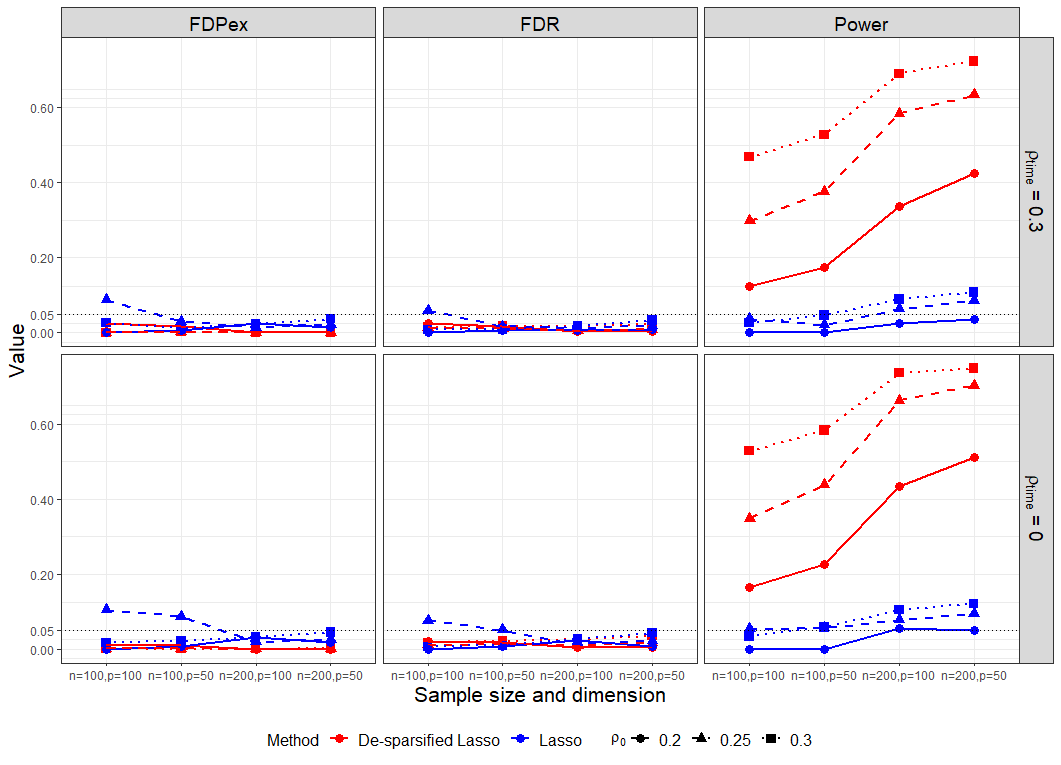
\includegraphics[width=\linewidth]{New-plot-lasso.png}
	\caption{The average FDPex rate $\mathbb{P}(\mbox{FDP} > 0.1)$, FDR and power of the proposed method with the lasso estimate (blue) and the de-sparsified lasso estimate (red) for testing the hypotheses (2.5) to recover the nonzero treatment effects on the subject level regression coefficients in Example 2 under the block-diagonal signal setting with $s_0 = 10$, $m = 300$, $n = 100, 200$, $p = 50, 100$ and $\rho_{\mathrm{\scriptstyle time}} = 0$ and $0.3$. The nominal level was $0.05$.}
	\label{simulation3}
\end{figure}

\begin{figure}[h]
	\centering
	
	\subfigure[Axial]{
		\begin{minipage}[t]{0.45\linewidth}
			\centering
			\includegraphics[width=3in]{Figures/Brain_Axial_causal.png}
		\end{minipage}
	} \ \ \
	\subfigure[Coronal]{
		\begin{minipage}[t]{0.45\linewidth}
			\centering
			\includegraphics[width=3in]{Figures/Brain_Coro_causal.png}
		\end{minipage}
	}
	\caption{Pairs of ROIs with significant treatment effects of medication on brain functional connectivity of ASD patients, measured by correlations among ROIs, by the proposed multiple testing procedure. The colors of nodes represent the functional networks they belong to.
	%SMN (red), Visual (orange), EAN (green), DMN (sky blue), SBN (purple) and Cerebellum (pink).
	}
	\label{Causalconnection}
\end{figure}


\end{document} 